
%!TEX root = ../thesis.tex
%*******************************************************************************
%*********************************** First Chapter *****************************
%*******************************************************************************

\chapter{Introduction}\label{chapter:introduction}  %Title of the First Chapter
\newcommand*\diff{\mathop{}\!\mathrm{d}} 



\makeatletter
\let\oldr@@t\r@@t
\def\r@@t#1#2{%
\setbox0=\hbox{$\oldr@@t#1{#2\,}$}\dimen0=\ht0
\advance\dimen0-0.2\ht0
\setbox2=\hbox{\vrule height\ht0 depth -\dimen0}%
{\box0\lower0.4pt\box2}}
\LetLtxMacro{\oldsqrt}{\sqrt}
\renewcommand*{\sqrt}[2][\ ]{\oldsqrt[#1]{#2}}
\makeatother


\ifpdf
    \graphicspath{{Chapter1/Figs/Raster/}{Chapter1/Figs/PDF/}{Chapter1/Figs/}}
\else
    \graphicspath{{Chapter1/Figs/Vector/}{Chapter1/Figs/}}
\fi



%TALK ABOUT SPEC-Z SURVEYS

 
\section{An overview of astronomical surveys}\label{section:surveys}
Astronomy, the study of the universe and its contents, is one of the oldest natural sciences. Across its rich history, from the first naked eye observations of the solar system to probing the edge of the observable universe, astronomical research has progressed through a combination of two methods. The first approach is to study an individual object, such as a star, planet or galaxy in detail. But the number of objects in the night sky is too large, and their variety too great, to investigate them all in this manner. The second approach, therefore, is to survey the sky to collect large samples. These samples can be used as a way to find new objects for detailed follow-up, or for statistical studies of populations. Generally speaking, progress in astronomy has often been pushed forward by the development of new observational tools \citep{2013pss2.book..223D}. With each new invention, a new frontier for science opens up. When this happens, surveys are often the first step in the exploration of the newly accessible regimes. \par


\subsection{A brief history of astronomical surveys}\label{subsection:history}
Following \cite{wynn2016surveying}, an insightful way to describe the history of astronomy is to focus on new technologies as a trigger for progress. With the discovery of each major observational toolkit, a new era of discovery opens up. \cite{wynn2016surveying} divides astronomy into five distinct historical epochs: 

\subparagraph{The Naked Eye Era} From BC to the invention of the telescope in the 17th century the sky was catalogued using only naked eye observations. This period saw the first record of what could be considered an astronomical survey: a star catalogue of 71 stars and constellations made by the Babylonians around the 8th century BC. 

\subparagraph{The Telescope Era} Galileo’s invention of the telescope in 1609 launched the beginning of a new form of astronomy. Telescopes allowed for much deeper observations, but objects still had to be recorded by hand. The \cite{1781cote.rept..227M} catalogue  and star counts by the Herschel family in the late 18th century are famous examples of important works from this period. 

\subparagraph{The Photographic Era} The third era started with the introduction of astrophotography around 1880. Using photographic plates, astronomers could make permanent records of their observations, and long exposures allowed them to probe much fainter objects. The Astrographic Catalogue and the Carte du Ciel were ambitious projects undertaken by a collaboration of 20 observatories between 1891 and 1950. Their purpose was to make a photographic map of the entire celestial sphere. Together with the Harvard Plate Collection (1885--1993), which repeatedly photographed the sky in search of variable stars, these could be considered the first instances of a survey in the modern sense of the word. Of all the photographic surveys throughout the epoch, the Palomar Observatory Sky Survey (POSS-I; 1949--1958; see \citealt{1963bad..book..481M}), was perhaps the most impactful. This project, covering two thirds of the sky, was made possible by the invention of Schmidt telescopes, which were especially well suited to taking the wide field exposures required for efficient surveying.

\subparagraph{The Electromagnetic Era} Up until the 1930s, all astronomy was carried out using visible light (with small extensions into the ultraviolet and infrared using special photographic plates). From the 1930s onwards, special detectors opened up the radio, X-ray, ultraviolet (UV), and infrared (IR) wavebands. Of particular interest to this thesis is the development of infrared astronomy, which studies radiation roughly from 1 $\mu$m to 1mm. The range from 1 $\mu$m to 2.5 $\mu$m is referred to\footnote{It must be emphasised that these definitions can differ between publications, and that the conventions listed here are the ones used in this thesis.} as the near-infrared\footnote{In physics the infrared region conventionally starts at 0.7$\mu$m, just beyond the reddest light visible with the naked eye; but in astronomy light between 0.7$\mu$m--1$\mu$m is generally imaged with the same instruments as visible light and is therefore often regarded as part of the optical waveband.}, 2.5 $\mu$m to 30 $\mu$m as the mid-infrared, 30 $\mu$m to 450 $\mu$m as the far-infrared, and 450 $\mu$m to 1 mm as the submillimeter. The IR branch of astronomy took off in the 1960s with the development of sensitive solid-state IR detectors. The Two Micron Sky Survey (TMSS; \citealt{1969tmss.book.....N}) was the first all-sky IR survey, imaging the whole sky in the near-IR at 2.2 $\mu$m (i.e. the present-day $K$-band). 

\subparagraph{The CCD Era} Several breakthroughs in digital technology and computing triggered the beginning of a fifth era of astronomy in the 1990s. Thanks to the enormous progress facilitated by these inventions, we are now firmly in a time where digital technology enables enormous surveys discovering sources by the billions. Several important developments in this period will be the primary focus of the current chapter. 

\subsection{Technological advancements: towards a data revolution}\label{subsection:technological_advancements}
With every new invention in each epoch, the capacity for generating observational data increased. The scientific potential of surveys was, however, often held back by limited ability to process all this data. For example, optical catalogues in the photographic era had to be compiled by hand, which restricted their size to at most several tens of thousands of objects. It was not until the 1990s, when the technology for scanning and digitising images became available, that the full potential of photographic surveys could be unlocked  \citep{1990AJ.....99.2019L,1998wfsc.conf...89D}. To give an example, after the POSS-II (the successor to the POSS; 1980s-1990s; \citealt{1991PASP..103..661R}) had been digitised, the scanned images contained \SI{3}{\TB} of pixel data. These generated a catalogue of $\sim 50$ million galaxies and $\sim 500$ million stars to limiting magnitudes of  $\sim \SI{22}{\mag}$ \citep{1998wfsc.conf...89D} --- a vast increase over the several tens of thousands of galaxies that could be recorded in catalogues compiled by hand. \par


Infrared astronomy was similarly also initially held back by limited data recording and processing capacity. The aforementioned TMSS from the 1960s illustrates these challenges very well. Signals for the eight lead sulfite detectors that made up the TMSS camera were recorded on multi-channel medical strip chart recorders, and source detection and measurements were carried out by eye. Another example comes from other experiments in the 1970s and 1980s with mid- and far-IR telescopes on sub-orbital rockets, which recorded \SI{25}{\MB} of data during 4 minutes of operation. The fact that this data took 5 hours to process, illustrates the enormous computing progress that needed to be made to enable the digital revolution of the CCD era. \par

By the end of the 1980s, however, a digital all-sky IR survey started to become technologically possible. Crucial factors were the release from military classification of solid-state infrared detectors suitable for astronomical research, as well as the availability of cheap computing to process the huge resulting data streams. The first two major digital IR surveys were the Two Micron All Sky Survey (2MASS; 1996--2001; \citealt{2006AJ....131.1163S}) and the Deep Near Infrared Survey of the Southern Sky (DENIS; 1997--2001; \citealt{1997Msngr..87...27E}). They covered the entire sky and the southern hemisphere respectively, both using cameras made up of an array of $256 \times 256$ detectors (i.e. pixels). Every one of these \num{56536} detectors was more sensitive than each one of the eight TMSS sensors, resulting in an \SI{11}{\mag} increase in depth over the TMSS (final survey depths were $K\sim 14.3$ for 2MASS and $K\sim14.0$ for DENIS). The increased sensitivity also facilitated a vast increase in the number of source detections: \num{470 000 000} and \num{355 000 000} for 2MASS and DENIS respectively vs. 5600 for the TMSS. \par

Meanwhile, optical astronomy surveys continued to rely largely on photographic plates. Nevertheless, by the early 1990s, the technology for a large digital project was finally beginning to converge in the optical regime as well, thanks to the invention of large-scale digital cameras with charged coupled device (CCD) chips, together with the development of cheap computing capabilities. In contrast to photographic surveys, which generally used several photographic plates sensitive to various colours, CCD cameras can image different colours in an automated fashion. This is achieved by applying a series of broadband filters (also called bands) that only transmit light within certain wavelength limits (this technique had already been employed in several digital IR surveys in the 1990s as well). The first major project to capitalise on all this new digital optical technology was the Sloan Digital Sky Survey (SDSS; 2000-ongoing; \citealt{2000AJ....120.1579Y}), which has since covered just over a third of the entire sky to depths of $r\sim 22.2$. Its 120 megapixel camera consists of an array of 30 CCDs of $2048 \times 2048$ pixels each, which has thus far been used to assemble an enormous catalogue of nearly one billion unique objects. As of 2019, the total data volume of the SDSS is over \SI{170}{\TB} \citep{2019ApJS..240...23A}. \par


Following on from these early successes, the CCD era of astronomy blossomed. With ever bigger and more advanced projects, astronomy is now well into the petascale data stream regime. For example, the Panoramic Survey Telescope and Rapid Response System (Pan-STARRS; 2010-ongoing; \citealt{2002SPIE.4836..154K}, \citealt{2010SPIE.7733E..0EK}) currently produces several \si{\TB} of data every night, and its most recent \SI{1.6}{\PB} data release from January 2019 is the largest in astronomical history. Using a 1.4 gigapixel camera, Pan-STARRS aims to image three quarters of the sky to $r\sim \SI{23.2}{\mag}$. A second example of a large modern optical survey is the Dark Energy Survey (DES; 2012--2019; \citealt{2005IJMPA..20.3121F}). This project currently constitutes the deepest large-scale survey in the southern hemisphere, having observed \SI{5000}{\sqdeg} to depths of $r\sim24.3$ with its 570 megapixel camera. After data processing will have been completed, its final total volume is expected to be around \SI{2}{\PB} \citep{2012SPIE.8451E..0DM}. \par

In the near-infrared, current state-of-the-art instruments include the United Kingdom Infrared Telescope (UKIRT) and the Visible and Infrared Survey Telescope for Astronomy (VISTA). With 16 megapixel and 67 megapixel  cameras respectively, both telescopes have carried out several large-scale surveys, ranging from footprints of approximately \SI{4000}{\sqdeg} to a full hemisphere  \citep{2007MNRAS.379.1599L,2013Msngr.154...35M,2018MNRAS.473.5113D}. The depths of these surveys reach up to $K\sim \SI{18.2}{\magvega}$ (UKIDSS on UKIRT)  and  $K_{s}\sim\SI{18.1}{\magvega}$ (VHS on VISTA). Such substantial increases in depths and camera sizes over 2MASS and DENIS has allowed these newest surveys to collect far larger numbers of objects. For instance, the wide galactic and extragalactic components of UKIDSS found 84 million galaxies and nearly a billion stars, an enormous gain compared to the $\lesssim500$ million sources for 2MASS and DENIS. \par

The data explosion of the last 30 years presently shows no signs of slowing down. Further telescopes are currently planned or under construction, the most prominent of which is probably the Large Synoptic Survey Telescope (LSST; \citealt{2008SerAJ.176....1I}). When completed, its 3.2 gigapixel camera will be the largest in the world, and it will aim to cover half the sky to a limiting magnitude of $r\sim27.7$ by taking many exposures in short succession. Every night LSST is expected to generate around \SI{20}{\TB} of data, which means that it would take just nine nights to surpass the entire SDSS data output. At the end of the project, the final volume of raw images will amount to \SI{60}{\PB}, and the corresponding \SI{15}{\PB} source catalogue is expected to contain 10 billion galaxies and a similar number of stars. \par

It is clear that  the digital revolution of the CCD era has changed astronomy from a relatively data-poor to an intensely data-rich discipline \citep{2013pss2.book..223D}. This transformation brings many new opportunities for research on ever larger and deeper datasets. The science generated by all these surveys so far has been very broad, and has covered cosmological research such as measurements of large-scale structure, dark matter, and dark energy; as well as galaxy evolution studies. On a smaller scale, research has included investigations of the oldest stars, brown dwarfs, the structure of the Milky Way, and dwarf galaxies. \par


\subsection{Deep-field surveys}\label{subsection:deep_field_surveys}
So far we have seen the amazing technological progress that has revolutionised astronomy by generating very large wide-area surveys. But sometimes, one can also discover a great deal from observing a smaller patch of the sky in detail. The main advantage of such narrower surveys is that they can dedicate much more exposure time to a specific region, which means that observations can go several magnitudes deeper. In some form, small but deep surveys have always existed. Indeed, nearly every telescope throughout history has at some point been pushed to its observational limit to see what lies at the edge. But the field of small-scale surveys truly took off with the space-based observations of the \textit{Hubble Space Telescope (HST)}. Its great success prompted a vast range of surveys from space, and later also from the ground. These projects, sometimes referred to as `deep fields', are almost always aimed at galaxy formation and evolution studies. Their observed area is too small for studies of large-scale cosmology, stars, and galactic structure, but they are ideal for finding distant galaxies, as deep imaging is needed to find these faint sources. \par


\subsubsection{Brief interlude on distances, redshifts and cosmic time}\label{subsubsection:redshift_interlude}
It is interesting to pause and reflect briefly on the scientific value of distant galaxies. Such objects are of primary interest to the study of galaxy evolution, because they can provide a window into the cosmic past. This is due to the finite speed of light, which causes the light from any astronomical source to take a non-zero amount of time to reach an observer. The observer therefore sees the object as it was in the past\footnote{A note from the author: I believe that this point ought to inspire a deep appreciation in anyone with a love for astronomy. The fact that looking further equates to looking earlier in time, is one of the most scientifically useful outcomes of the laws of physics. And yet it is not a necessary truth that the universe is this way; it is a lucky coincidence of sorts, that the universe we live in happens to be one with a finite light speed. --- A. L. S.}. This concept implies a result that is deeply entrenched in modern astronomy, yet in essence highly profound: \textit{in studying galaxies with increasing distance one can probe increasingly far into the cosmic past.} Because this connection is of crucial importance to this thesis, the current section presents a number of important related principles and quantities. \par


First of all, \textit{redshifts} provide a means of measuring distances to faraway galaxies. Due to the expansion of the universe, objects that are moving away from an observer solely due to this expansion (i.e. moving with the so-called Hubble flow) recede with increasing relative velocity the more distant they are \citep{1929PNAS...15..168H}. The light emitted by such an object is Doppler-shifted, and this shift can be captured by a dimensionless quantity called redshift. The redshift $z$ of such a source is defined as:

\begin{equation}
    z \equiv \frac{\lambda_{\mathrm{obs}}-\lambda_{\mathrm{em}}}{\lambda_{\mathrm{em}}} = \frac{\lambda_{\mathrm{obs}}}{\lambda_{\mathrm{em}}}-1, \label{eqn:redshift_definition}
\end{equation}

\noindent where $\lambda_{\mathrm{em}}$ is the wavelength emitted in the rest frame of the moving object, and $\lambda_{\mathrm{obs}}$ is the wavelength in the rest frame of the observer.  \par


Via the standard model of cosmology, the redshift of an object resulting from cosmic expansion can be linked to the lookback time $t_L$, which is the difference between the age of the universe at the point of observation (i.e. now), and the age of the universe when the object emitted the observed photons (\citealt{1999astro.ph..5116H} following \citealt{1993ppc..book.....P}) : 

\begin{equation}
    t_L(z)= \frac{1}{H_{0}} \int_{0}^{z} \frac{ \diff z'}{(1+z')\sqrt{\Omega_{R}(1+z')^4+\Omega_{M}(1+z')^3+\Omega_{k}(1+z')^2+\Omega_{\Lambda}}}.\label{eqn:lookback_time}
\end{equation}


\begin{figure}[t] 
\centering    
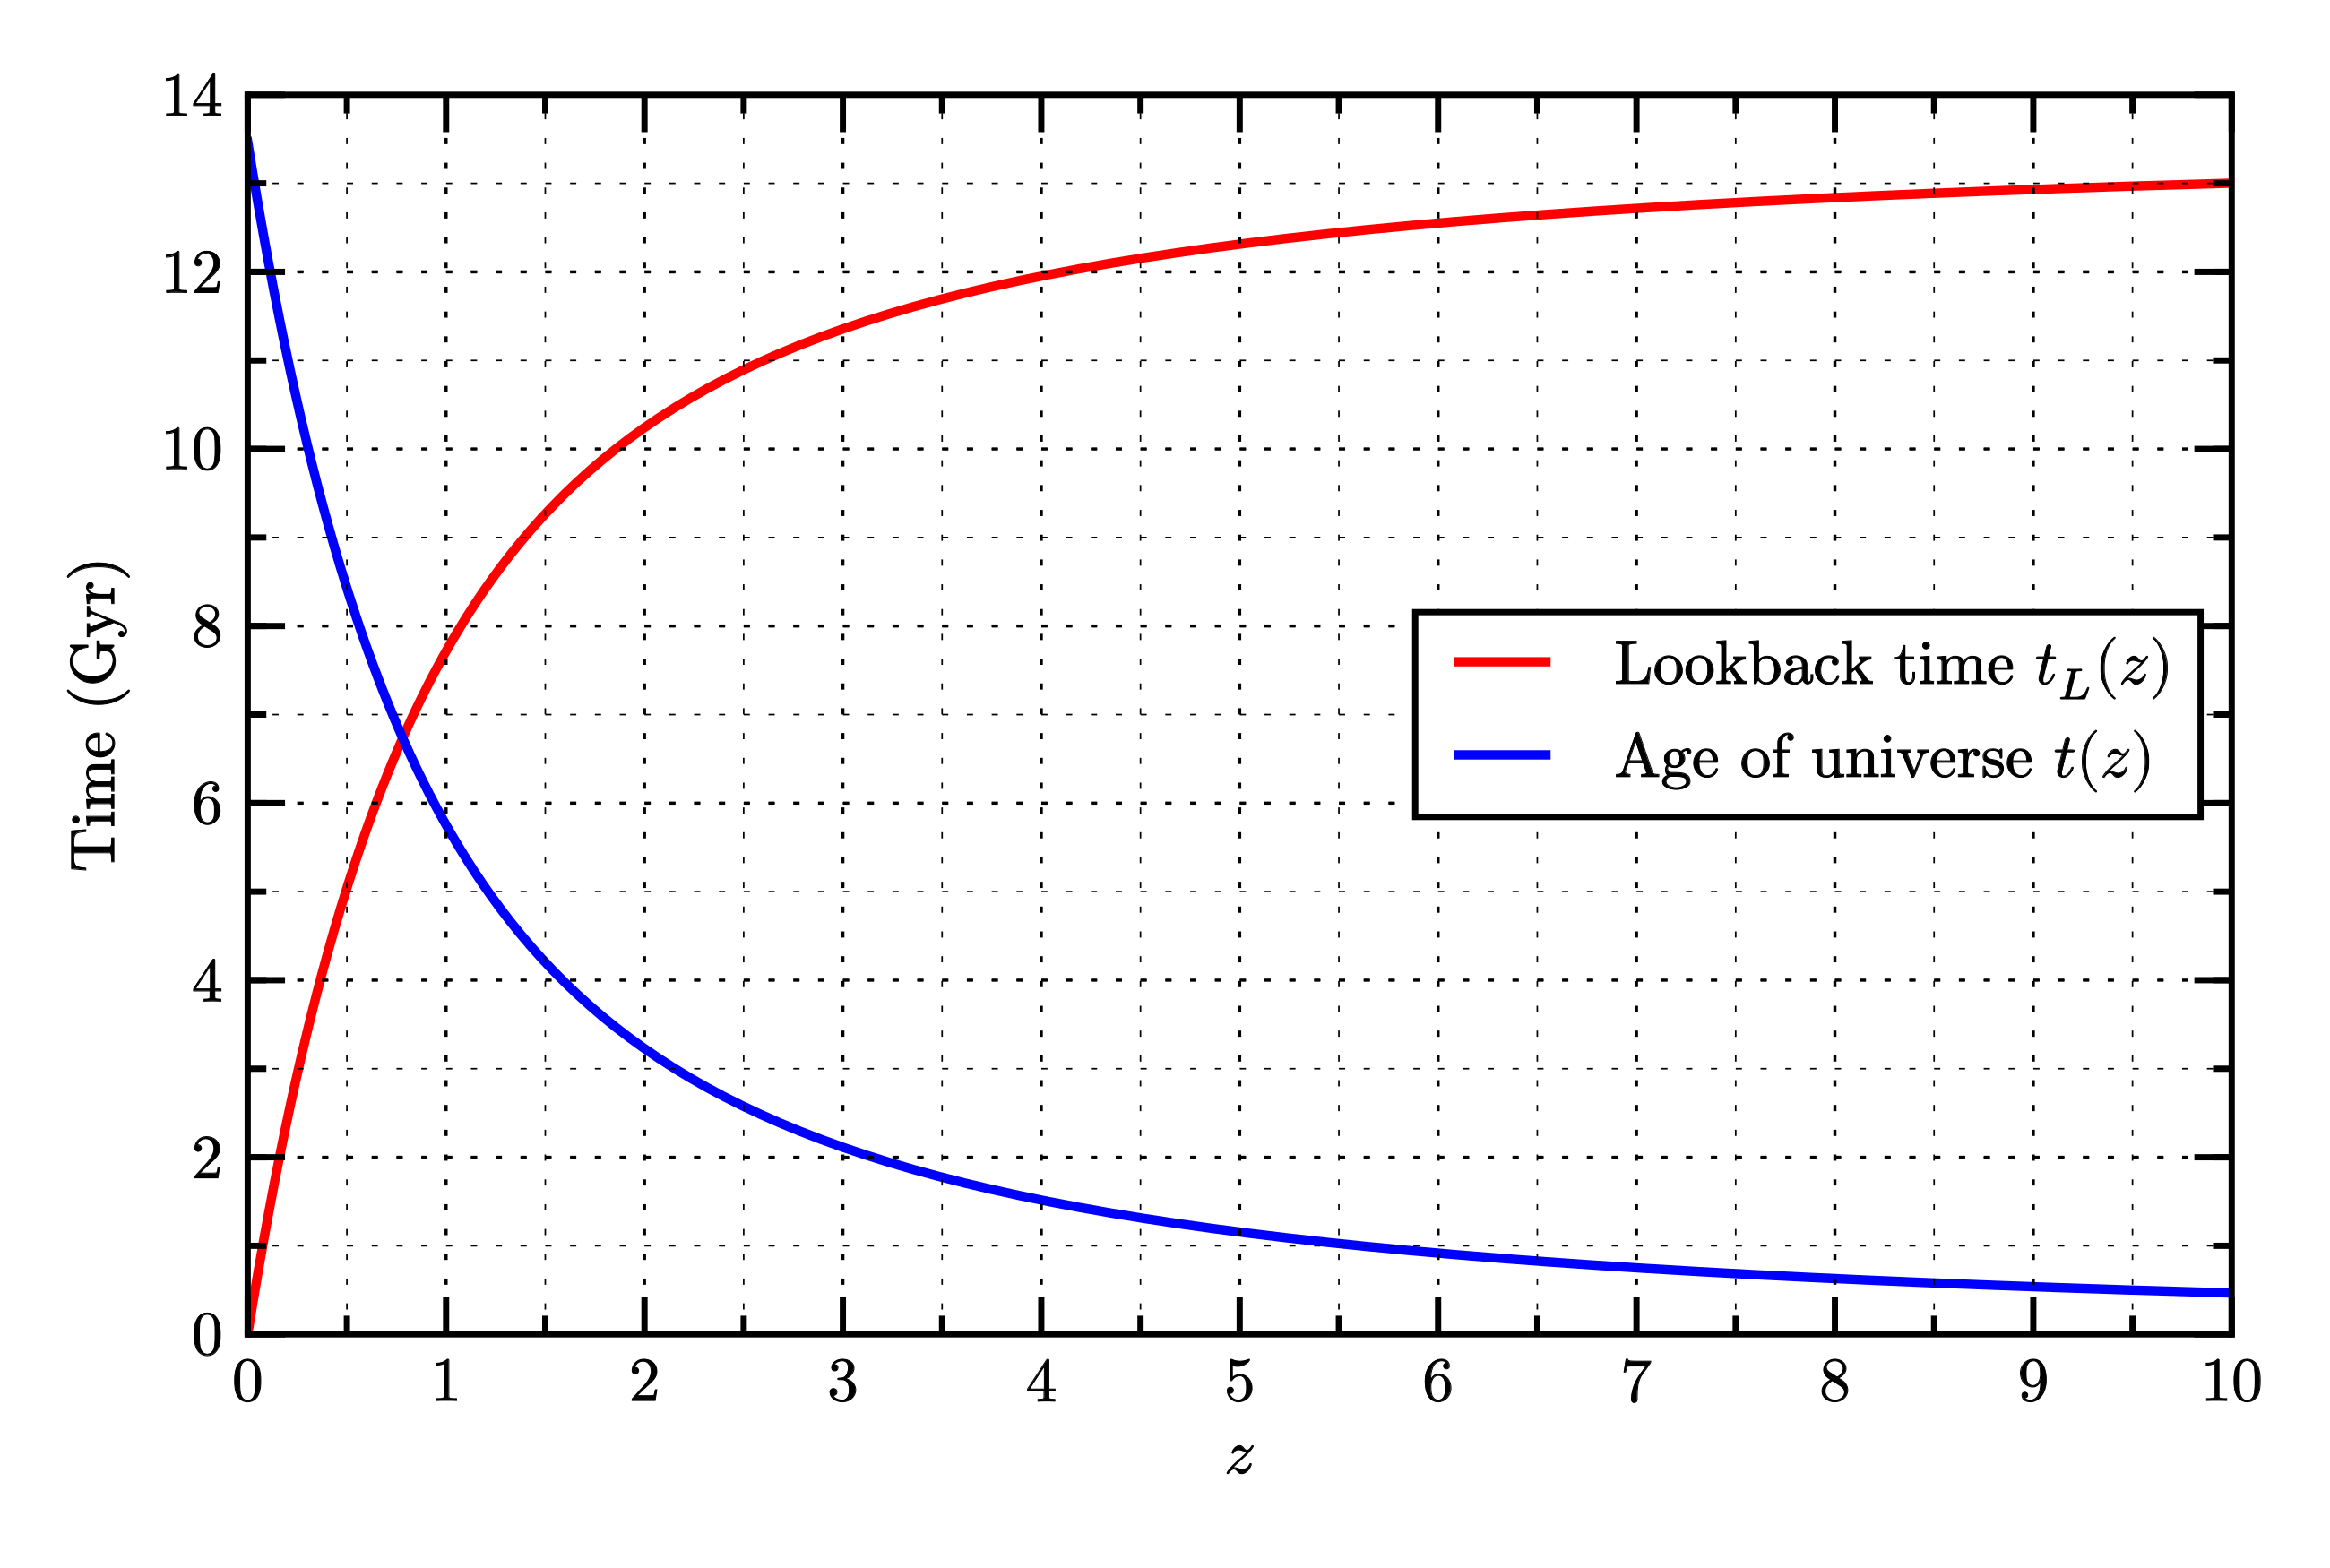
\includegraphics[width=0.95\textwidth]{Chapter1/Figs/lookback_time.png}
\caption[Relation between redshift and cosmic time]{The lookback time $t_L(z)$ and age of the universe $t(z)$ for an object observed at a redshift $z$, provided that its redshift is purely caused by cosmic expansion.} 
\label{fig:lookback_time}
\end{figure}

\noindent Here $\Omega_{R}$ is the present-day radiation density, $\Omega_{M}$ is the present-day total matter density, $\Omega_{\Lambda}$ is the present-day dark energy density, $\Omega_{k}=1-\Omega_{M}-\Omega_{\Lambda}$ is the curvature, and $H_{0}$ is the Hubble constant. Throughout this thesis, all calculations will assume\footnote{Even though the assumption of $\Omega_{R}=0$ is not strictly true, it is an excellent approximation in the matter-dominated era  with which this thesis is concerned, as measurements have shown that $\Omega_{R}\simeq 0.8 \times 10^{-4}$ \citep{2008ARA&A..46..385F}.} a cosmology of $\Omega_{M} = 0.3$, $\Omega_{\Lambda} = 0.70$, $\Omega_{R}=0$ and $H_{0} = \SI{70}{km.s^{-1}.Mpc^{-1}}$. In addition to the lookback time, the age of the universe $t$ when the light from an object at redshift $z$ was emitted can be found by changing the integration boundaries in Equation \ref{eqn:lookback_time} \citep{2008ARA&A..46..385F}: 

\begin{equation}
    t(z)= \frac{1}{H_{0}} \int_{z}^{\infty} \frac{ \diff z'}{(1+z')\sqrt{\Omega_{R}(1+z')^4+\Omega_{M}(1+z')^3+\Omega_{k}(1+z')^2+\Omega_{\Lambda}}}.
\end{equation}

To visualise the relation between cosmic time and redshift, the lookback time and age of the universe\footnote{A note from the author: it is interesting to note that the lookback time increases incrementally slowly with increasing redshift. The fact that the laws of physics cause this behaviour is highly serendipitous; it results in an extremely useful set of circumstances in which the history of the universe can be studied with increasing resolution further back in time. In this way, the redshifts of the very earliest galaxies provide a very precise handle to study the build-up of cosmic structure. --- A. L. S. } are both plotted as a function of redshift in Figure \ref{fig:lookback_time}.  \par




\paragraph{Measuring redshifts} 
The equations above illustrate why redshifts are so important to galaxy evolution studies: if it is possible to obtain redshift measurements, galaxies can be sorted by cosmic epoch, so that changing properties can be studied statistically as a function of time.  As implied by Equation \ref{eqn:redshift_definition}, redshifts can be found by comparing the wavelengths of certain features in an observed, i.e. redshifted, galaxy spectral energy distribution (SED) to their corresponding expected rest-frame wavelengths. The most precise way to do this involves spectroscopy, comparing the observed wavelengths of certain emission or absorption lines in a high-resolution spectrum to the wavelengths of these transitions as measured in a laboratory. Some astronomical surveys, such as the SDSS, incorporate this technique via a spectroscopic component  \citep{2012AJ....144..144B}. There have also been other projects that are exclusively spectroscopic, targeting galaxy candidates that have been selected from other imaging surveys (e.g. \citealt{2001MNRAS.328.1039C, 2005ApJ...620..595W,2005A&A...439..845L}).  \par

However, as will be discussed in more detail in Section \ref{section:photometric_redshifts}, obtaining spectra is time-consuming, and unfeasible for the huge catalogues produced by modern surveys. Nevertheless, even without a high-resolution spectrum that exhibits individual absorption or emission lines, it is often still possible to use colours from broadband filters to obtain an approximate redshift estimate. Examples of this method include photometric redshifts (see Section \ref{section:photometric_redshifts}) and colour cuts (exclusively for objects at $z\gtrsim3$; see Section \ref{subsubsection:lyman_break}). In this way, the redshifts of galaxies in the enormous surveys of the CCD era can be estimated using only the survey data itself.  \par


\subsubsection{Small area space-based surveys}\label{subsubsection:space_based_surveys}
With the power of distance measurements provided by redshift estimates, deep-field surveys can be an extremely powerful tool for galaxy evolution studies. The current section briefly reviews the developments in this fast-moving field of research.  \par


\afterpage{\newpage\begin{ThreePartTable}
\begin{TableNotes}
\item[] \hspace{-0.5em} \textbf{References}: \\
\item[i] \cite{1994AAS...185.5309G}
\item[ii] \cite{1996AJ....112.1335W}
\item[iii] \cite{2000AJ....120.2747C}
\item[iv] \cite{2004ApJ...600L..93G}
\item[v] \cite{2006AJ....132.1729B}
\item[vi] \cite{2005AJ....130....1T}
\item[vii] \cite{2013ApJS..209....6I}
\item[viii] \cite{2007ApJS..172....1S}
\item[ix] \cite{2007ApJ...660L...1D}
\item[x] \citealt{2011ApJS..197...35G, 2011ApJS..197...36K}

\vspace{0.5em}
\item[] \hspace{-0.5em} \textbf{Other comments}: \\
\item[a] The HXDF is assembled out of all Hubble data in the HUDF region. 

\item[] \hspace{-0.3em}\textit{Almost all fields in this table have been studied in several wavelengths since being released, but}
\item[] \hspace{-0.3em}\textit{the following projects contained further multiwavelength data as part of their core science goals:}
\item[b] Also contains X-ray, mid-IR, far-IR data; and ground-based optical, near-IR data. 
\item[c] Also contains X-ray, UV, mid-IR, far-IR data; and ground-based optical, near-IR, radio data.
\end{TableNotes}

\renewcommand\TPTminimum{\textwidth}
\setlength{\tabcolsep}{0.15em}
\centering
\footnotesize
\begin{longtable}{lcccccccccc}
\multicolumn{11}{c}{\normalsize \textsc{Small-scale space-based optical and near-infrared surveys}}\\
\toprule\toprule 
\endhead
\midrule\midrule
\multicolumn{11}{r}{\textit{continued}}
\endfoot
\insertTableNotes \\
\bottomrule\\
\caption[Small-scale space-based surveys]{Overview of major small-scale space-based surveys over optical (`visible'/`vis) and near-infrared (`NIR') wavelengths.}\label{table:space_small_survey}\\
\endlastfoot


Survey & Type & Epoch & Area &  \multicolumn{5}{c}{Bands, depth} & \si{\magab} & \textnumero{} galaxies \\
\midrule

GSS\tnote{i} & Visible & 1994 & \SI{127}{\sqarcmin} & \multicolumn{5}{c}{\begin{tabular}[t]{cc} $V_{606}$ & $I_{814}$ \\ 26.1 & 25.4 \end{tabular}} & $5\sigma$ & 11 000 \\ 
%Groth \cite{1994AAS...185.5309G}

HDF\tnote{ii} & Visible & 1995 & \SI{6.25}{\sqarcmin} & \multicolumn{5}{c}{\begin{tabular}[t]{cccc} $U_{300}$  & $B_{450}$ & $V_{606}$ & $I_{814}$ \\ 27.0 & 27.9 & 28.2 & 27.6  \end{tabular}} & $10\sigma$ & 3000 \\

HDF-S\tnote{iii} & Visible & 1998 & \SI{6.25}{\sqarcmin} & \multicolumn{5}{c}{\begin{tabular}[t]{cccc} $U_{300}$  & $B_{450}$ & $V_{606}$ & $I_{814}$ \\ 26.8 & 27.7 & 28.3 & 27.7  \end{tabular}} & $10\sigma$ & 2700 \\

GOODS\tnote{iv} & Visible\tnote{b} & 2002--2003 & \SI{320}{\sqarcmin} & \multicolumn{5}{c}{\begin{tabular}[t]{cccc} $B_{435}$ & $V_{606}$ & $i_{775}$ & $z_{850}$ \\ 27.8 & 27.8 & 27.1 & 26.6 \end{tabular}} & $10\sigma$ & 73 000  \\

HUDF\tnote{v} & Visible & 2003--2004 & \SI{11}{\sqarcmin} & \multicolumn{5}{c}{\begin{tabular}[t]{cccc} $B_{435}$ & $V_{606}$ & $i_{775}$ & $z_{850}$ \\ 29.1 & 29.5 & 29.4 & 28.7  \end{tabular}} & $10\sigma$ & 10 000 \\

NICMOS UDF\tnote{vi} & NIR & 2003 & \SI{5.8}{\sqarcmin} & \multicolumn{5}{c}{\begin{tabular}[t]{cc} $J_{110}$ & $H_{160}$  \\ 27.7 & 27.7  \end{tabular}} & $5\sigma$ & 1300 \\

%TALK ABOUT THIS IN THE TEXT

HXDF\tnote{vii,a} & Vis-NIR & 2002--2013 & \SI{11}{\sqarcmin} & \multicolumn{5}{c}{\begin{tabular}[t]{ccccc} $B_{435}$ & $V_{606}$ & $i_{775}$ & $I_{814}$ &  $z_{850}$ \\ 29.8 & 30.3 & 30.3 & 29.1 & 29.4 \\ \multicolumn{5}{c}{\begin{tabular}[t]{cccc} $Y_{105}$ & $J_{125}$ & $JH_{140}$ & $H_{160}$ \\ 30.1 & 29.8 & 29.8 & 29.8 \end{tabular}} \end{tabular}} & $5\sigma$ & 14 000\\


COSMOS\tnote{viii} &  {\begin{tabular}[t]{c} Visible\tnote{c} \\ \\ Visible\tnote{c} \\ \\ NIR\tnote{c} \\ \\ \end{tabular} } & 2003--2005 & {\begin{tabular}[t]{c} \SI{1.8}{\sqdeg} \\ \\  \SI{1.07}{\sqdeg} \\ \\ \SI{330}{\sqarcmin} \\ \\ \end{tabular}} &
\multicolumn{5}{c}{\begin{tabular}[t]{cc} $g_{475}$ & $I_{814}$ \\ 27.9 & 27.5 \\ $U_{300}$ & $B_{450}$ \\ 24.8 & 26.7 \\ \multicolumn{2}{c}{$H_{160}$} \\ \multicolumn{2}{c}{ 25.9 } \end{tabular}}   & $5\sigma$ &  {\begin{tabular}[t]{c} 1 700 000 \\ \\ \\ \\ 21 000  \\ \\ \end{tabular}} \\ 

AEGIS\tnote{ix} & {\begin{tabular}[t]{c} Visible\tnote{c} \\ \\ NIR\tnote{c} \\ \\ \end{tabular} } & 2004--2005 &  {\begin{tabular}[t]{c} \SI{700}{\sqarcmin} \\ \\ \SI{46}{\sqarcmin} \\ \\ \end{tabular}} & \multicolumn{5}{c}{\begin{tabular}[t]{cc} $V_{606}$ & $I_{814}$ \\ 28.1 & 27.5 \\ $J_{110}$ & $H_{160}$ \\ 25.7 & 25.5 \end{tabular}} & {\begin{tabular}[t]{c} $5\sigma$ \\ \\ $10\sigma$ \\ \\ \end{tabular} } & {\begin{tabular}[t]{c} 80 000 \\ \\ 4000 \end{tabular}}  \\ 

CANDELS\tnote{x} & Vis-NIR & 2010--2013 &  \multicolumn{5}{c}{} & & $5\sigma$  & 250 000 \\

\multicolumn{1}{l}{\textit{Wide}} & & & \SI{770}{\sqarcmin} & \multicolumn{5}{c}{\begin{tabular}[t]{ccc} \multicolumn{3}{c}{\begin{tabular}[t]{cc}  $V_{606}$ & $I_{814}$ \\ 27.6 & 27.5 \end{tabular} } \\ \multicolumn{3}{c}{ \begin{tabular}[t]{ccc}  $Y_{105}$ & $J_{125}$ & $H_{160}$  \\ 26.6 & 26.4 & 26.5 \end{tabular} } \\\end{tabular}} &  & \\

\multicolumn{1}{l}{\textit{Deep}} & & & \SI{120}{\sqarcmin} & \multicolumn{5}{c}{\begin{tabular}[t]{ccccc}  $B_{435}$ & $V_{606}$ & $i_{775}$ & $I_{814}$ & $z_{850}$ \\ 27.8 & 28.2 & 27.5 & 28.4 & 27.3 \\ 
\multicolumn{5}{c}{ \begin{tabular}[t]{ccc}  $Y_{105}$ & $J_{125}$ & $H_{160}$  \\ 27.3 & 27.4 & 27.2 \end{tabular} } \\  \end{tabular}} &  & \\

\end{longtable}
\end{ThreePartTable}
}



The prototype for the modern concept of extremely deep fields is the Hubble Deep Field (HDF; \citealt{1996AJ....112.1335W}), imaged by the \textit{HST}. The space-borne nature of this instrument makes it especially well suited to extremely deep imaging. Because it avoids blurring by the Earth's atmosphere, images can be more detailed and deeper, as light is spread out over fewer pixels. The HDF contains 3000 galaxies with magnitudes of up to $V \sim \SI{30}{\mag}$ for the faintest sources, and several objects with redshifts of $z>5$. The Hubble Ultra Deep Field (HUDF; \citealt{2006AJ....132.1729B}) and the Hubble Extreme Deep Field (HXDF; \citealt{2013ApJS..209....6I}) imaged the same region of the sky as the original HDF, over larger areas and with newer cameras. These surveys achieved even higher depths and pushed the discovery of high-redshift galaxies to $z\sim7$ and $z\sim12$ respectively, reaching the very limit of what is possible with current technology. Table \ref{table:space_small_survey} presents a summary of some core properties of the Hubble Deep Field surveys. \par 



After the success of the Hubble Deep Fields, further deep \textit{HST} surveys followed.   Progress was mainly made in the direction of larger areas and more wavelength coverage. This helped to build up a more comprehensive picture of galaxy evolution, as the larger size of the observed fields allowed the assembly of larger, statistically significant samples to study changes in galaxy populations. Table \ref{table:space_small_survey} summarises several noteworthy examples of these surveys. Each one specialised in a specific redshift regime, but together they cover cosmic time between roughly $0.5\lesssim z \lesssim 8$. Examples of galaxy properties that have been studied with these datasets include mass assembly, the coupled evolution of galaxies, active galactic nuclei (AGN), and large-scale structure. The bigger sample sizes also facilitated applications in cosmology, such as studies of dark matter through gravitational lensing. \par  


\subsubsection{Intermediate-area ground-based surveys}\label{subsubsection:ground_based_surveys}
A major downside to space-based surveys is that the main optical and near-IR instrument is the \textit{HST}, which has a very restricted amount of available observing time and a limited field of view compared to ground-based telescopes. On top of that, ground-based telescopes are more cost-effective for larger surveys, especially for areas over $\sim \SI{1}{\sqdeg}$. To capitalise on these advantages, astronomers have started to conduct intermediate-area deep surveys from the ground, often utilising the sophisticated terrestrial instruments developed during the CCD revolution (described in Section \ref{subsection:technological_advancements}).  Such intermediate surveys cover several square degrees, to much higher depths than the large-scale wide-area projects from Section \ref{subsection:technological_advancements}. In this way, they can cover much more area than space-based ones, although they are generally not quite as deep and have much lower image resolution due to atmospheric blurring. \par 


\afterpage{\newpage\begin{ThreePartTable}
\begin{TableNotes}
\item[] \hspace{-0.5em} \textbf{References}: \\
\item[i] \cite{1999ASPC..191..111J}
\item[ii] \cite{2002SPIE.4836...73W}
\item[iii] \cite{2004PASJ...56.1011K}
\item[iv] \cite{2008ApJS..176....1F}
\item[v] \cite{2012AJ....143...38G}
\item[vi] \cite{2007MNRAS.379.1599L}
\item[vii] \cite{2013MNRAS.428.1281J}
\item[viii] \cite{2012A&A...544A.156M}
\item[ix] \cite{2012ApJ...753..152B,2016MNRAS.460.1270D}


\vspace{0.5em}
\item[] \hspace{-0.5em} \textbf{Other comments}: \\
\item[a] Because galaxy counts were not provided, these are total source counts. \\
\item[b] These are the expected final depths for point sources from the full five years of observations. They differ from the depths for the DES data presented later in this thesis (Table \ref{table:actual_des} and Figure \ref{fig:area_depth}), which are for a \SI{1.95}{\arcsec} aperture using only the first year of observations. 
\end{TableNotes}

\renewcommand\TPTminimum{\textwidth}
\setlength{\tabcolsep}{0.15em}
\centering
\footnotesize
\begin{longtable}{lcccccccccc}
\multicolumn{11}{c}{\normalsize \textsc{Intermediate-scale ground-based optical and near-infrared surveys}}\\
\toprule\toprule 
\endhead
\bottomrule
\multicolumn{11}{r}{\textit{continued}}
\endfoot
\insertTableNotes \\
\bottomrule\\
\caption[Intermediate-scale ground-based surveys]{Overview of major intermediate-scale ground-based surveys over optical (`visible'/'vis') and near-infrared (`NIR') wavelengths.}\label{table:ground_small_survey}\\ 
\endlastfoot

Survey & Type & Epoch & Area &  \multicolumn{5}{c}{Bands, depth} & \si{\magab} & \textnumero{} galaxies \\
\midrule

NDWFS\tnote{i} & Vis-NIR & 1997--1999 & \SI{9}{\sqdeg} & \multicolumn{5}{c}{\begin{tabular}[t]{cccc} $B_{w}$ & $R$ & $I$ & $K$ \\ 27.2 & 26.3 & 25.9 & 21.0 \end{tabular}}  & $5\sigma$ & 3 200 000\tnote{a} \\

DLS\tnote{ii} & Visible & 2001--2006 & \SI{20}{\sqdeg} & \multicolumn{5}{c}{\begin{tabular}[t]{cccc} $B$ & $V$ & $R$ & $z'$ \\ 26.6 & 26.5 & 26.9 & 24.8  \end{tabular}} & $5\sigma$ & 5 000 000 \\
%\cite{2002SPIE.4836...73W} 

%\cite{1999ASPC..191..111J}
SDF\tnote{iii} & Visible & 2002--2004 & \SI{920}{\sqarcmin} & \multicolumn{5}{c}{\begin{tabular}[t]{ccccc} $B$ & $V$ & $R$ & $i'$ & $z'$ \\ 28.5 & 27.7 & 27.8 & 27.4 & 26.6  \end{tabular}} & $3\sigma$ & 210 000 \\
%\cite{2004PASJ...56.1011K}

SDXF\tnote{iv} & Visible &  2002--2005 & \SI{1.2}{\sqdeg} & \multicolumn{5}{c}{\begin{tabular}[t]{ccccc} $B$ & $V$ & $R_{c}$ & $i'$ & $z'$ \\ 28.4 & 27.8 & 27.7 & 27.7 & 26.6  \end{tabular}} & $3\sigma$ & 900 000\tnote{a} \\

CFHTLS-D\tnote{v} & Visible & 2003--2009 & \SI{4}{\sqdeg} & \multicolumn{5}{c}{\begin{tabular}[t]{ccccc} $u*$ & $g'$ & $r'$ & $i'$ & $z'$ \\ 27.5 & 27.9 & 27.9 & 27.7 & 26.5 \end{tabular}} & $5\sigma$ & > 300 000 \\

UKIDSS-UDS\tnote{vi} & NIR & 2005--2012 & \SI{0.77}{\sqdeg} & \multicolumn{5}{c}{\begin{tabular}[t]{ccc} $J$ & $H$ &  $K$ \\ 26.3 & 26.0 & 25.6  \end{tabular}} & $5\sigma$ & 250 000 \\

UKIDSS-DXS\tnote{vi} & NIR & 2005--2012 & {\begin{tabular}[t]{c}  \SI{35}{\sqdeg} \\ \\ \SI{5}{\sqdeg} \\ \end{tabular}} & \multicolumn{5}{c}{\begin{tabular}[t]{cc} $J$  &  $K$ \\ 23.4 & 22.9 \\ \multicolumn{2}{c}{$H$} \\ \multicolumn{2}{c}{23.4} \end{tabular}} & $5\sigma$ & 3 000 000\tnote{a} \\
%\cite{2007MNRAS.379.1599L}


VIDEO\tnote{vii} & NIR & 2009--2018 & \SI{12}{\sqdeg} & \multicolumn{5}{c}{\begin{tabular}[t]{ccccc} $Z$ & $Y$ & $J$ & $H$ & $K_{s}$ \\ 25.7 & 24.5 & 24.4 & 24.1 & 23.8 \end{tabular}} & $5\sigma$ & 1 700 000\tnote{a} \\
%\cite{2013MNRAS.428.1281J}

UltraVISTA\tnote{viii} & NIR & 2009--2018 & \multicolumn{5}{c}{}  & & $5\sigma$ & 200 000\tnote{a} \\

\multicolumn{1}{l}{\textit{Deep}} & & & \SI{1.5}{\sqdeg} & \multicolumn{5}{c}{\begin{tabular}[t]{cccc} $Y$ & $J$ & $H$ & $K_{s}$ \\ 24.8 & 24.5 & 24.1 & 23.8 \\  \end{tabular}}  &  & \\

\multicolumn{1}{l}{\textit{Ultra-Deep}} & & & \SI{0.73}{\sqdeg} & \multicolumn{5}{c}{\begin{tabular}[t]{cccc} $Y$ & $J$ & $H$ & $K_{s}$ \\ 25.7 & 25.4 & 25.1 & 24.1 \\  \end{tabular}}  &  & \\

DES Deep\tnote{ix}\tnote{b} & Visible & 2013--2019 & & \multicolumn{5}{c}{} & $5\sigma$ & 2 000 000 \\

\multicolumn{1}{l}{\textit{Shallow}} & & & \SI{24}{\sqdeg} & \multicolumn{5}{c}{\begin{tabular}[t]{cccc} $g$ & $r$ & $i$ & $z$ \\  27.7  & 26.5 & 26.8 & 26.6  \\  \end{tabular}}  &  & \\

\multicolumn{1}{l}{\textit{Deep}} & & & \SI{6}{\sqdeg} & \multicolumn{5}{c}{\begin{tabular}[t]{cccc} $g$ & $r$ & $i$ & $z$ \\  28.0 & 28.2 & 27.9 & 27.7  \\  \end{tabular}}  &  & \\

\end{longtable}
\end{ThreePartTable}
}



Their position between the shallow wide-area ground-based surveys and the ultra-deep narrow space-based surveys makes intermediate-scale surveys ideal for intermediate applications. As will be illustrated in more detail below, they are often used to collect larger samples than possible with space-based surveys, in order to improve sample statistics. Furthermore, they are more likely to contain rare objects that require a larger search area. Intermediate-scale surveys can also unveil cosmological structures larger than the few Mpc scales probed by space-based surveys, and can reduce biases introduced by cosmic variance. On top of that, they offer a significant increase in lookback time over wide-area surveys. Their major downside is that they are not able to reach quite as high redshifts as the space-based datasets, so they generally cannot be used to find the  utmost distant sources. \par

%at the same time, they offer...

%For many intermediate-scale surveys, a larger observational footprint has offered significant scientific advantages. 

Table \ref{table:ground_small_survey} lists several important examples of intermediate-scale surveys. For many of these, a larger observational footprint has offered significant scientific advantages. A common research goal has been to collect large samples for improving population statistics. For instance, the Subaru Deep Field (SDF) survey revealed statistically significant samples of Lyman-break galaxies at $z \approx \numrange{4}{5}$ and Lyman-$\alpha$ emitters at $z \approx \numrange{5}{6} $. Similarly, the UKIDSS Deep Extragalactic Survey (UKIDSS-DXS) aimed to facilitate a statistical study of galaxy properties at $z\sim 1$, to compare with the $z\sim 0$ picture from local surveys such as SDSS. Furthermore, UltraVISTA has enabled a representative study of the peak of star formation at $2<z<3$, and the VISTA Deep Extragalactic Observations (VIDEO) survey has been targeted at providing a comprehensive view of the evolution of galaxies with their environment out to $z\approx4$. A second commonly occurring goal of the surveys in question has often involved finding uncommon objects. Rare object searches have included AGN searches in the VIDEO survey, the deep component of the Canada-France-Hawaii Telescope Legacy Survey (CFHTLS-D), and the NOAO Deep Wide Field Survey (NDWFS). Additionally, the most luminous galaxies can be studied at $3<z<5$ in the CFHTLS-D, at $z>4$ in the NDWFS, and out to $z\approx7$ in UltraVISTA and the UKIDSS Ultra-Deep Survey (UKIDSS-UDS). Ultravista was also designed to uncover galaxies at the highest redshifts ($ z \simeq 6.5--9$). A third aim of some ground-based surveys, such as the Dark Energy Survey Deep Fields and CFHTLS-D, has been to look for Type Ia supernovae to constrain dark energy. Lastly, the fourth major application of intermediate-scale surveys concerns studies of large-scale structure for the purpose of constraining cosmological parameters. Examples include the Subaru Deep XMM-Newton Survey (SDXF), NDWFS, and the Deep Lens Survey (DLS), the latter of which specifically focused on weak gravitational lensing. \par 



\subsection{Multiwavelength datasets}\label{subsection:multiwavelength}
Many of the astronomical surveys that have been discussed often cover a particular wavelength regime, generally  optical or near-infrared. Their scientific successes show that each such dataset can be incredibly powerful on its own. However, in many cases, combining observations from surveys over multiple wavebands can open up further opportunities for interesting discoveries. \par 
%SMOOTHE IT UP

Historically, the combination of surveys over a wide range of the electromagnetic spectrum has been very fruitful. Perhaps the oldest and simplest application of such a multiwavelength approach is the use of optical data for the identification of sources that were discovered in other frequencies. For instance, in the early ages of infrared and radio astronomy, the physicists that pioneered these fields often turned to the optical POSS-I survey (see Section \ref{subsection:history}) for this purpose. Other historical examples where combining datasets from different wavelengths has revealed results that could not be recognised in a single dataset alone include the discovery of quasars (QSOs) and ultraluminous starbursts, and the interpretation of $\gamma$-ray bursts (see \citealt{2013pss2.book..223D}). \par


To capitalise on the opportunities offered by multiwavelength astronomy, contemporary observations are often coordinated between instruments specialising in different wavelength regimes. In particular, several of the small and intermediate area surveys from Tables \ref{table:space_small_survey} and \ref{table:ground_small_survey} have been designed as part of a collaboration of different instruments, and some others have later been followed up at other wavelengths. These developments are moving astronomy into a regime where the energetic output of a source can be traced throughout large parts of the electromagnetic spectrum. The study of galaxy evolution is one research area that particularly benefits from the great scientific power of panchromatic datasets, and the following two sections will present two examples. \par 

\subsubsection{Uncovering galaxy properties with multiwavelength data}
The first asset of a multiwavelength approach is that different frequencies trace different galaxy properties. To name a few examples, optical imaging unveils their positions and morphologies, as well as possible environmental disruptions such as mergers with neighbouring objects \citep{2010MNRAS.401.1043D,2017MNRAS.464.4176W}. Near-infrared data can be valuable as well, for instance for measuring stellar masses \citep{2003ApJS..149..289B}. Furthermore, X-ray, mid-infrared, and radio observations can detect AGN, including those obscured by dust \citep{2018ARA&A..56..625H}. X-ray data can also be used to find hot intergalactic gas around galaxy mergers and clusters \citep{2006ApJ...643..692C,2018MNRAS.475.2067B}. Finally, information from the ultraviolet, mid-IR, and radio wavebands can track the rate of active star formation \citep{2017ApJ...847..136B}. \par 

The wavelength regimes listed above generally apply to the rest-frame emission. When objects are redshifted, the wavebands required to trace certain galaxy properties will become redder. For instance, as will be discussed in detail in Section \ref{subsubsection:lyman_break}, galaxies generally show a sharp break at (rest-frame) wavelengths of $\lambda=\SIrange{912}{1216}{\angstrom}$, emitting very little flux below this cutoff. At $z>6$, this cutoff is redshifted to $\lambda>\SI{8500}{\angstrom}$, so sources at these distances will emit almost all their flux in the observed near-infrared and beyond. Therefore, imaging at $\lambda> \SI{8500}{\angstrom}$ will be needed to observe them at all. Furthermore, properties which are locally measured at UV wavelengths, such as the star formation rate, are traced by observed-frame near-IR imaging at these high redshifts. \par

 
\subsubsection{The benefits of multiwavelength data for estimating redshifts}\label{subsubsection:multiwavelength_redshifts}

The second core strength of multiwavelength datasets involves improved redshift estimates from broadband colours. Such measurements generally rely on several strong spectral features in galaxy rest-frame UV and optical emission (most importantly the Lyman limit at $\lambda = \SI{912}{\angstrom} $, the $\lambda=\SI{1216}{\angstrom}$ break, the Balmer break at $\lambda=\SI{3646}{\angstrom}$, and the $\lambda = \SI{4000}{\angstrom}$ break). However, with increasing redshift, these features will trivially shift towards longer wavelengths, so that redder imaging becomes more and more important. For instance, at $z>1.5$ the \SI{4000}{\angstrom} break has redshifted out of the optical and into the near-IR. Secondly, as mentioned earlier, beyond $z>6$ the observed emission from galaxies --- and hence all their important spectral features --- lies almost entirely in the near-IR and beyond. Therefore, near-infrared imaging is almost always necessary to determine redshifts for $z>6$ galaxies  \citep{2009MNRAS.395.2196M,2014MNRAS.440.2810B}. This point will be revisited later in Section \ref{subsubsection:lyman_break_galaxy_history}. \par




A particularly common method for estimating redshifts in modern astronomy is the so-called photometric redshift technique. An in-depth discussion of this method will follow shortly in Section \ref{section:photometric_redshifts}, where it will be shown that this is a highly effective technique for obtaining redshift estimates from broadband fluxes in large surveys. The photometric redshift approach essentially computes the redshift of a given object by using its broadband colours as a very low resolution spectrum. Simple statistics prima facie dictate that adding data in more filters will improve the resulting redshift estimates, simply by increasing the amount of available information. The most striking example of this is perhaps the photometric redshift catalogue for the COSMOS field \citep{2009ApJ...690.1236I}. With 30 broadband colours covering the UV, optical, near-IR, and mid-IR, the accuracy of this panchromatic dataset approaches that of spectroscopic redshifts (when compared with spectroscopic redshifts $\Delta z= z_{\mathrm{spec}} - z_{\mathrm{phot}}$, the dispersion is $\sigma_{\Delta z/ (1+z_{\mathrm{spec}})} =0.007$ for sources brighter than $i^{+}_{\mathrm{AB}}<22.5$).  Furthermore, several simulations \citep{2008MNRAS.386.1219B,2008MNRAS.387..969A} and observational studies \citep{2009ApJ...690.1236I,2013MNRAS.428.1281J,2015MNRAS.446.2523B} have indicated that photometric redshift estimates benefit from including infrared data in particular.  Altogether, it is therefore clear that combining surveys from multiple wavebands is beneficial to galaxy evolution studies (as well as many areas of astronomy in general). \par 


\subsection{Conclusion on surveys}\label{subsection:conclusion_surveys_intro}
We have now reached the end of our birds-eye-view journey through survey astronomy, which forms the first part of the introduction to this thesis. Along the way, we have seen how advances in technology and instrumentation have given rise to a situation where celestial sources can now be discovered electronically millions or billions at a time. Thanks to this data-driven revolution, the last 30 years can undoubtedly be characterised as the CCD era of astronomy. This period has witnessed large-scale wide surveys imaging substantial parts of the sky, as well as smaller deeper surveys unveiling increasingly distant cosmic structures. We have also seen how combining observations over multiple wavelength regimes can often increase the scientific potential of surveys even further. The enormous datasets resulting from all of these developments have led to many new discoveries across several branches of astronomy, and there are doubtlessly many more to come. \par 

But the explosion of data also comes with certain obstacles. Some of these, such as the infrastructure needed to process the gigantic data streams, lie within the realm of technology and computer science. Other challenges are computational and astrophysical in nature, and concern the extraction of physically meaningful quantities from survey data.It is aspects from the latter category that the current text will address. \par

%It is aspects from the latter category that the current work {\color{red}has taken up}.

%

%As part of this, the first part of this thesis will focus on the task of combining

%As part of this, the first part of this thesis will address the task of combining optical and near-infrared data from two deep intermediate-area ground-based surveys to create a single, more powerful multiwavelength catalogue.

As part of this, the first part of this thesis will focus on the task of combining optical and near-infrared data from two deep intermediate-area ground-based surveys to create a single, more powerful multiwavelength catalogue. This new merged data product can harness the potential of panchromatic datasets, creating a useful resource for the rest of this thesis as well as for the scientific community. The next part of the thesis will then describe the process of acquiring distance estimates for all objects in the catalogue. This is achieved through photometric redshifts, and this computational method forms the topic of the next part of this introduction.  \par




\section{Photometric redshifts}\label{section:photometric_redshifts}
Many branches of research in modern extragalactic astronomy rely crucially on distance measurements. As mentioned previously in Section \ref{subsubsection:redshift_interlude}, spectroscopic redshifts generally offer the most accurate way of doing this. However, for a multitude of reasons that will be discussed imminently, it is not always feasible to measure redshifts spectroscopically. To circumvent this problem, photometric redshifts (photo-zs) can be measured from broadband magnitudes only. The idea is simple: multiband photometry is essentially a very low resolution spectrum, and can therefore be used to estimate redshifts \citep{1998astro.ph..9347Y}. Primarily, this tactic relies on broad spectral features that exist in the emission of most galaxies (predominantly the Lyman break at $\lambda = \SIrange{912}{1216}{\angstrom}$ and the Balmer/\SI{4000}{\angstrom} break). The photometric redshift approach has two major strengths: 

%GENERALLY=ON THE WHOLE

\begin{enumerate}
    \item Photometric redshifts can be computed for a far larger number of objects than is feasible with spectroscopy. The catalogues of modern surveys in the CCD era can contain millions or billions of galaxies. Despite the efficiency of modern multi-object spectrographs, it is only possible to measure meaningful spectra for a few percent of these sources, as spectroscopy is relatively time-consuming \citep{2005A&A...439..845L,2019NatAs...3..212S}. On the other hand, broadband magnitudes can be extracted directly from the imaging, which is obtained for all objects in the field of view simultaneously. The remaining problem of estimating the photo-zs is computational in nature, but the time required for this is minimal compared to the duration of spectroscopy. The latter issue is especially pressing for high-redshift research, as even the most luminous galaxies at redshifts $z \sim 6$ are so faint that they require integration times of several hours (e.g. \citealt{2013AJ....145....4W}). This makes spectroscopy an unfeasible method to search for such distant sources, which are extremely rare compared to the abundance of low-redshift galaxies. 
    
    \item The photometric redshift method can be used on sources for which conventional spectroscopy is not possible. As it relies only on broadband magnitudes, the technique can be applied to all galaxies in a given source catalogue, including objects with very low apparent brightness all the way out to a survey's imaging limits \citep{1998astro.ph..9347Y,2019NatAs...3..212S}. These faint sources that lie outside the current realm of spectroscopy include very small galaxies or galaxies at extremely high redshifts. 
\end{enumerate}

\noindent These two advantages have made the use of photometric redshifts ubiquitous for large datasets, and the method has become an integral part of data processing in galaxy surveys \citep{2013ApJ...775...93D}. The following sections will give a historical overview of the development of photo-zs and discuss specific techniques available in the literature. \par

\subsection{Historical overview}\label{subsection:photoz_history}
\cite{1962IAUS...15..390B} was the first ever author to use broadband photometry for estimating galaxy redshifts. He computed photo-zs by comparing magnitudes in nine photometric filters to spectra from galaxies in the Virgo cluster.  After that, the next occurrence of the photometric method was not until the 1980s, when it was once again employed by several authors. Butchins (\citeyear{1981A&A....97..407B}, \citeyear{1983MNRAS.203.1239B}), \cite{1982ApJ...257L..57P}, and \cite{1985AJ.....90..418K} all estimated photometric redshifts by comparing colours from photographic plates to those derived from template galaxy SEDs. Midway through the decade, \cite{1986ApJ...303..154L} first pioneered the use of CCD photometry. After these initial developments, the photometric redshift method remained relatively unused for the next 10 years, but from the middle of the 1990s it experienced a resurgence. The main reasons for this revival were twofold:

 


\begin{itemize}
    \item As the data revolution of the CCD era took off in the 1990s, broadband photometry could suddenly be obtained efficiently for huge samples of galaxies. The object counts of the resulting source catalogues were far too high to perform spectroscopy for every object, so it became necessary to use a more efficient method for distance measurements. In order to meet this need, many authors turned to photometric redshifts. 
    
    \item The publication of the HDF (see Section \ref{subsubsection:space_based_surveys}) provided a dataset containing galaxies with magnitudes out to $V \sim \SI{30}{\magab}$. Such sources are far too faint for conventional spectroscopy, necessitating the use of photometric redshifts. 
\end{itemize}


    
With these factors as impetuses for further development and refinement of the photo-z approach, many papers followed soon after (e.g. \citealt{1995AJ....110.2655C,1997ApJ...482L..21B,1998AJ....116.2081W,1996Natur.381..759L,1996ApJ...468L..77G,1996A&A...314...73P}). As the number of existing surveys and their source counts continued to rise while the CCD era advanced, the use of photometric redshifts grew even more widespread. More codes became available in the literature, and the available methods became more sophisticated. These developments will shortly be detailed further in Section \ref{subsection:methods}, which will describe in detail the variety of codes that have been created over the last three decades.  As the use of photometric redshifts became standard practice, many scientists started to make their photo-z methods publicly available. The first such public code was \texttt{HyperZ} \citep{2000A&A...363..476B}. Many others soon followed, including \texttt{BPZ} \citep{2000ApJ...536..571B},  \texttt{ANNz} \citep{2004PASP..116..345C},  \texttt{ZEBRA} \citep{2006MNRAS.372..565F},  \texttt{LePHARE} \citep{2006A&A...457..841I,2011ascl.soft08009A}, \texttt{EAZY} \citep{2008ApJ...686.1503B}, \texttt{ArborZ} \citep{2010ApJ...715..823G}, \texttt{TPZ} \citep{2013MNRAS.432.1483C,2010ApJ...712..511C} and \texttt{GPz} \citep{2016MNRAS.462..726A}. \par 


\subsection{Methods}\label{subsection:methods}
\cite{2011Ap&SS.331....1W} and \cite{1998astro.ph..9347Y} identify two main photometric redshift strategies commonly used in the literature. \textit{Empirical methods} employ a subset of objects with measured spectroscopic redshifts as a training set. This subset is used to determine an empirical relation between (spectroscopic) redshift and galaxy properties such as colour and magnitude. Photometric redshifts are then inferred by applying this relation to the entire dataset. \textit{Template methods} use pre-existing galaxy spectral energy distributions --- also known as templates --- from models or libraries of observed spectra. These SEDs can be stretched to any redshift, and predicted magnitudes can be computed by convolving the shifted SEDs with the transmission curves used in the relevant survey. For each object, all the predicted magnitudes are then compared to the observed photometry to find the best-fitting redshift and template combination. The following two sections will describe both empirical and template methods in more detail. \par 


\subsubsection{Empirical methods}\label{subsubsection:empirical_methods}
As mentioned above, empirical methods rely on a training sample to  calibrate a relation $z=z(C,m_{0})$ between redshift $z$ and observed colours $C$ or magnitudes $m_{0}$ \citep{2000ApJ...536..571B}. The phrase empirical refers to the fact that this relation is derived empirically from data in the training sample  only. \par 

The first empirical methods were developed when photometric redshifts rose to prominence in the mid-1990s. These early approaches were simple yet powerful. Even fitting functions $z=z(C,m_{0})$ where $z$ is a linear function or simple polynomial proved effective at estimating redshifts when appropriately tuned \citep{1995AJ....110.2655C}. For example, \cite{1998AJ....116.2081W} computed photo-zs via a linear relationship between redshift and three photometric colours ($U-B$, $B-V$, and $V-I$). The simple polynomial approach was applied successfully by e.g. \cite{1995AJ....110.2655C}, who fitted a second order polynomial to $U$, $B_{J}$, $R_{F}$ and $I_{N}$ magnitudes, and by \cite{1997ApJ...482L..21B}, who employed an iterative process with several quadratic functions of $U$, $B$, $R$, and $I$ magnitudes. \par

Early such forms of the empirical method proved superior to template methods \citep{2011Ap&SS.331....1W} for a number of reasons. Firstly, because the training set consists of real galaxies, there can be no issues with inaccurate templates. On top of that, the empirical relation is calibrated using magnitude measurements from survey data, so it inherently accounts for the effects of filter bandpasses and flux calibrations. Empirical methods can also easily provide realistic estimates of redshift uncertainties \citep{2011Ap&SS.331....1W}, and they generally outperform template methods in terms of speed as well \citep{2004A&A...423..761V,2019NatAs...3..212S}.  \par

A disadvantage of the empirical approach is that the derived relation $z=z(C,m_{0})$ is only valid for the full survey if the training set is representative, that is, if the training set has similar observables $C$ and $m_{0}$ to the full survey. This can be an issue when calculating photo-zs for objects much fainter than the training set (such as at high redshifts), because the relation has to be extrapolated in those cases.  Another problem is that galaxies at redshifts beyond those in the training sample may have different intrinsic SEDs. A further,  related drawback is that the sample also needs to be large enough to cover all colours, magnitudes, galaxy types, and redshifts to a statistically significant degree, so that the inferred empirical relation is statistically sound. \par

Empirical photo-z codes have become more advanced since the early methods described before, making use of sophisticated computational techniques which have developed alongside the field of machine learning. The core idea of these approaches is still the same as for the simple early methods: through machine learning, a training set is used to build up a relationship  between survey observables and redshifts. Examples of specific algorithms include decision tree classification (e.g. \texttt{ArborZ}), random forests (e.g. \texttt{TPZ}), support vector machines (e.g. \citealt{2005PASP..117...79W}), Gaussian processes (e.g. \texttt{GPz}), and Neural Networks (e.g. \texttt{ANNz}).  Machine learning techniques inherit all the strengths and weaknesses of the early empirical methods listed above. However, they also enjoy the additional advantage of being able to include other observables on top of the standard photometry. Examples include the bulge-to-total flux ratio \citep{1999ApJS..121..417S}, surface brightness \citep{2007AJ....134.1360K}, Petrosian flux radius \citep{2004PASP..116..345C}, and concentration index \citep{2004PASP..116..345C}. \par


\subsubsection{Template methods}\label{subsubsection:template_methods}
Unlike the empirical strategy, which makes use of a spectroscopic training set, the template method computes photometric redshifts by directly comparing the observed photometry to a library of pre-existing SEDs. These SEDs can be empirical templates (widely used template sets include those by  \citealt{1980ApJS...43..393C} and \citealt{1996ApJ...467...38K}), or theoretical models (such as \citealt{2003MNRAS.344.1000B}).  \par

All of the earliest photo-z implementations discussed in Section \ref{subsection:photoz_history} were variations on the template fitting method. The pioneering work by \cite{1962IAUS...15..390B}, and the studies by Butchins (\citeyear{1981A&A....97..407B}, \citeyear{1983MNRAS.203.1239B}) and \cite{1986ApJ...303..154L} all used empirical spectra. In the mid-1980s, theoretical templates were first introduced by \cite{1985AJ.....90..418K}. That decade also saw the first implementation of a $\chi^2$ minimisation procedure for template fitting  (\citealt{1982ApJ...257L..57P}; see Section \ref{subsubsection:chi_minimisation} for a detailed example of how $\chi^2$ minimisation works in the context of a specific photo-z code). Such $\chi^2$ algorithms, or variations thereof, have since become the most popular computational technique for contemporary template-based studies, and they are used in all subsequent papers and codes mentioned in this section.  \par


Following on from this early period, template methods remained in frequent use when photometric redshifts became increasingly popular during the start of the CCD revolution in the 1990s.  Significant works from this period include studies by \cite{1996Natur.381..759L}, \cite{1996ApJ...468L..77G} and \cite{1999ApJ...513...34F}, who all capitalised on the newly available deep photometry from the Hubble Deep Field. Soon after, a large number of authors created many more template fitting codes, which were often made available for public use. Prominent examples are \texttt{HyperZ}, \texttt{BPZ},  \texttt{ZEBRA},  \texttt{LePHARE}, and \texttt{EAZY}, and many of these still remain in frequent use to the current day. \par 


Compared to the empirical approach, a major asset of the template method is that it works even if there is no sufficient training set available. For this reason, template fitting codes are the preferred option when exploring new regimes, such as in new survey datasets that do not yet have large training sets available, or at high redshifts and faint magnitudes beyond the spectroscopic limit \citep{2011Ap&SS.331....1W,2017ApJ...838....5L}.  Additionally, a further advantage of template fitting is that it can be performed in a fully probabilistic fashion, with explicit priors over redshifts and types of galaxies \citep{2000ApJ...536..571B,2017ApJ...838....5L}. The outputs of some machine learning codes could also be interpreted in probabilistic terms, but their priors are often complicated and implicitly constructed from training data, rather than specified explicitly. Furthermore, the template method allows additional physical properties such as ages or star formation rates to be obtained directly from the best-fit SEDs \citep{2011Ap&SS.331....1W,2017ApJ...838....5L}. It must be noted, though, that some machine learning codes can predict these properties as well, given a suitable training set (see e.g. \citealt{2004MNRAS.348.1038B}). \par


The primary issues with the template fitting method lie with the template library, which needs to be representative of all galaxies in the survey. This is particularly an issue for theoretical model SEDs, which may not be entirely correct, and could be affected by specific details in the treatment of properties such as emission lines or dust reddening \citep{2011Ap&SS.331....1W}. It is also important that the template set is complete, i.e. that it spans the entire colour space of galaxies in the survey. Empirical templates are most susceptible to this problem; firstly because empirical libraries contain a limited number of SEDs, and secondly because the spectra they are measured from are local and thus potentially intrinsically different from higher redshift galaxies at a different evolutionary stage \citep{2011Ap&SS.331....1W}. \par 

Another drawback of the template fitting technique is that it cannot fully capture flux complexities such as biases or error underestimation \citep{2010MNRAS.405..987B,2017ApJ...838....5L}. These are exactly the types of situations where the empirical photo-z methods discussed in the previous section excel, as they can easily adapt to imperfect flux measurements. Some template fitting methods such as  \texttt{LePHARE}, \texttt{EAZY}, and \texttt{GOODZ} \citep{2010ApJ...724..425D} attempt to deal with this problem by adding correction terms to existing templates, or by adopting very flexible templates. For instance,  \texttt{LePHARE} and \texttt{GOODZ} incorporate some of the strengths of empirical methods to mitigate the imperfect flux problem: they use a training set of galaxies to derive corrections to  zero-points (\texttt{LePHARE}) or template SEDs (\texttt{GOODZ}) that minimise the scatter between photometric and spectroscopic redshifts. Nonetheless, these fixes often do not achieve the accuracy level attained by empirical codes. They can also be computationally expensive \citep{2017ApJ...838....5L}, although it must be remarked that the latter is not a problem when using small- or intermediate-scale surveys, for instance when hunting for high-redshift galaxies in deep surveys over relatively small areas. \par

Furthermore, colour-redshift degeneracies, which occur when the colours of a galaxy can be well fitted by SEDs at multiple redshifts, also present a challenge for photometric redshifts in general. They can be particularly problematic for template fitting codes, especially if the template set contains too many SEDs. Empirical codes can mostly circumvent the issue by breaking the degeneracy with additional information from magnitudes (or other observables for more recent machine-learning type codes). However, template methods have also found a way to deal with the problem via the use of Bayesian statistics. Through this framework, extra information can be included in the form of prior probabilities, which quantify the known likelihood of observed properties like galaxy shapes, angular sizes or magnitudes as a function of (measured spectroscopic) redshift. This extra information can break the degeneracy, because after incorporating prior probabilities one redshift solution will generally have a higher posterior probability than the others. In some cases, this could potentially even give template fitting codes an edge over the empirical approach, since it is possible to determine priors independently from the survey or field for which the photo-zs are to be computed.  In fact, many codes include pre-computed priors from previous, well-established spectroscopic fields. Lastly, a Bayesian interpretation of SED fitting can also retrieve redshift probability functions. Template methods that utilise those can produce accurate photo-z uncertainties, allowing such codes to catch up with empirical codes regarding realistic errors. Bayesian statistics and prior probabilities were first implemented in \texttt{BPZ} by \cite{2000A&A...363..476B}, and have since been included in many other codes (out of the ones mentioned in this chapter, specifically  \texttt{ZEBRA},  \texttt{LePHARE}, \texttt{EAZY}, and \texttt{GOODZ}). \par

\subsubsection{Comparison}\label{subsubsection:intro_comparison}
Whether an empirical or template fitting approach would be more suitable for a given dataset depends on the specific application and the availability of spectroscopic redshifts. In those cases where a complete and representative sample of spectroscopic redshifts is available, empirical codes perform better \citep{2011MNRAS.417.1891A,2019NatAs...3..212S}. Empirical codes are also not subject to photometry biases, and are therefore better if the aim is to reduce the impact of such biases, provided of course that a good sample of spectra is available. Finally, the fact that empirical methods are computationally faster provides a distinct advantage for the most massive datasets. This can be a strong asset for the enormous contemporary large-scale surveys. On the other hand, in deep surveys over small areas which extend out to very high redshifts (where there is insufficient spectroscopic coverage), template fitting codes should be favoured \citep{2010A&A...523A..31H}. Regarding the performance of specific codes, \cite{2010A&A...523A..31H} and \cite{2011MNRAS.417.1891A} provide a detailed comparison of several publicly available photo-z methods, both template and empirical --- although it is interesting to note that these two studies failed to identify a single best-performing code in either category. \par 
 

\subsection{Applications}\label{subsubsection:photoz_applications_intro}
The main drawback to the speed and efficiency of the photometric redshift strategy is a reduction in accuracy compared to spectroscopy. Photo-zs have larger errors on the redshift measurements, and they are subject to a greater risk of gross misestimation for a small number of individual objects (so-called catastrophic outliers). This can be a problem in areas where accuracy or certainty are of the utmost importance. However, since quantity is a quality of its own, for many scientific applications the reduced accuracy is an acceptable trade-off. Subsequently, photometric redshifts have become a key tool in many branches of extragalactic astronomy. This introduction cannot possibly do justice to all the existing applications in this extremely rich and fast-moving field, but some key examples will be presented briefly below. \par 


\subsubsection{Cosmology}
Because they facilitate the statistical analysis of large bodies of galaxies, photometric redshifts have become essential in large parts of observational cosmology \citep{2008ApJ...686.1503B}. By mapping out the positions of galaxies through broad regions of space across cosmic time, photo-zs provide valuable information about cosmological large-scale structure \citep{2006ewg3.rept.....P,2007MNRAS.374.1527B,2009ApJ...701...32S,2013PhR...530...87W,2013MNRAS.435.3017D,2018PhRvD..98d3526A,2018PhRvD..98d2006E,2019PASJ...71...43H}. This large-scale structure, in turn, can provide a handle on dark energy and dark matter, and provide a better understanding of the geometry, composition, evolution, and fate, of the universe. The digital revolution of the CCD era has played a crucial role in facilitating this research, and will continue to do so for the foreseeable future. Several current and future large-scale modern cosmology surveys, such as the SDSS, DES, Hyper Suprime-Cam Subaru Strategic Program (HSC-SSP; \citealt{2018PASJ...70S...4A}), and LSST are dedicated towards collecting broadband photometry for billions of objects, from which photometric redshifts can derive cosmological parameters. \par 


\subsubsection{Galaxy evolution}\label{subsubsection:photoz_galaxy_evolution}
As suggested previously in Section \ref{subsubsection:redshift_interlude}, redshift estimates can also be used to select samples of galaxies in specific cosmic epochs, so that changes in their properties can be traced throughout the history of the universe. In this way, the photo-zs of galaxies in large multiwavelength datasets have long been used to study evolving galaxy populations (e.g. \citealt{2000AJ....120.2206F,2012ApJ...756..164F,2014ApJ...792...76B}). The time evolution of galaxy sizes \citep{2000ApJ...530L..73G}, their UV spectral slopes \citep{2012ApJ...756..164F},  and their star formation rates \citep{2007ApJ...670..156D, 2013A&A...556A..55I} are examples of the types of properties that have been traced in this way.  The luminosity function (LF), which gives the number density of galaxies per unit of comoving volume per unit luminosity \citep{2013ASSL..396..223D}, is a common method of summarising changing galaxy demographics. Photometric redshifts can be used to determine the LFs at different redshifts, which, for instance, can be used to study changes in the abundances of bright or faint galaxies (e.g. \citealt{2003ApJ...593L...1P,2011AJ....142...41R,2010MNRAS.403..960M}). By comparing these observational luminosity functions to results obtained from models, it is also possible to obtain insights into the physical processes that drive this evolution. The scientific value of the LF will be illustrated further in Section \ref{subsubsection:high_redshift_galaxy_evolution}, specifically in the context of galaxies at $z\gtrsim5$. \par 



\subsection{Conclusion on photometric redshifts}\label{subsection:conclusion_photoz_intro}
Altogether, we have thus far witnessed clearly how, thanks to their computational efficiency, photometric redshifts have become an excellent way to extract important information out of datasets from modern surveys. Thanks to that valuable quality, this way of estimating cosmic distances now forms a crucial tool for many types of extragalactic astronomy. A core part of this thesis therefore concerns computing photo-zs for the optical+near-IR catalogue outlined earlier in Section \ref{subsection:conclusion_surveys_intro}. \par 

The objective of this work is threefold. Firstly, since photometric redshifts have become so vital to astronomy, it is valuable to study how to optimise their application. For instance, it is important to investigate the effect of the many different code options that we have seen in Section \ref{subsection:methods}.  The optical+near-IR catalogue from this thesis can provide a good testing ground for such tests. Notably, the catalogue also enables an investigation of the extent to which photometric redshifts improve with the addition of near-infrared data, a result suggested by several theoretical (e.g. \citealt{2008MNRAS.386.1219B}, \citealt{2008MNRAS.387..969A}) and observational studies (\citealt{2009ApJ...690.1236I}, \citealt{2013MNRAS.428.1281J}, \citealt{2015MNRAS.446.2523B}). With projects such as LSST and the \textit{James Webb Space Telescope} (\textit{JWST}; \citealt{2006SSRv..123..485G}) set to continue the progression in survey area and depth for at least the next 10 years, photo-zs will remain an extremely important area of study in the coming decades.  With regard to the future, insights on how to perfect their accuracy are thus highly valuable scientifically. Secondly, because of their many applications in astronomy, providing photometric redshifts for the aforementioned optical+near-IR catalogue further increases the value of this dataset for the scientific community in general. Lastly, another core aim of this thesis, which will be introduced in the next part of this introduction, is to search for $z\gtrsim5$ galaxies in the new optical+near-IR dataset. Because a photometric redshift strategy is ideally suited to identifying such objects (which we have previously noted often lie beyond the spectroscopic limit), photo-zs form a vital part of this endeavour.  \par



%\subsubsection{The search for {\color{red}high redshift} objects}
%Due to their capacity to handle huge numbers of sources, photometric redshifts are highly suitable for finding rare objects in large datasets. Interesting examples include recent findings of $6<z<7$ quasars  \citep{2017MNRAS.468.4702R,2019MNRAS.484.5142P,2019arXiv190107456R}, and extremely distant galaxies at $8<z<11$ \citep{2010MNRAS.403..960M,2013ApJ...763L...7E,2013ApJ...762...32C,2015MNRAS.450.3032M}. Particularly interesting is the $z\approx9.6$ candidate that was identified by \cite{2012Natur.489..406Z} based on its photometric redshift was later spectroscopically confirmed at  $z=9.11$ \citep{2018Natur.557..392H}. At the time of writing, a $z=11.1$ object found by \cite{2014ApJ...786..108O}, is currently the highest spectroscopically confirmed galaxy in the universe \citep{2016ApJ...819..129O}. Even though it was not primarily discovered on the basis of its photometric redshift, \cite{2014ApJ...786..108O} did make use of SED fitting to corroborate its high redshift. 


\section{High-redshift galaxies}\label{section:high_redshift_galaxies}
Returning briefly to the topic of modern surveys, Sections \ref{subsection:deep_field_surveys} and \ref{subsection:multiwavelength} have described how the impressive advance of deep field imaging over multiple wavelength regimes has opened the distant universe up to astronomers. Throughout this thesis, unless otherwise stated, the phrase `high-redshift' is used to refer to far-away sources at $z\gtrsim5$, and closer objects are denoted as `low-redshift'. By observing sources at those high redshifts, astronomers are beginning to catch a glimpse of the formation of galaxies in the first billion years of cosmic time. The fact that we are now able to probe such very early times could perhaps be considered one of the most impressive achievements of survey astronomy. The current part of this chapter will now introduce this rapidly advancing field.  \par




\subsection{Selection methods}\label{subsection:high_z_selection_methods}
Compared to the general population of celestial objects, high-redshift galaxies are faint, which makes it extremely time-consuming to measure their spectra, if they are bright enough that this is possible at all. Their faintness, compounded with the fact that they are also extremely rare, rules out spectroscopy as a feasible way to find $z\gtrsim5$ sources. To overcome this obstacle, an arsenal of several alternative search strategies has been developed in the literature. As Section \ref{section:photometric_redshifts} suggested at the start, photometric redshifts are indeed one possibility. The following sections will present several other search methods, and place the photo-z approach within this general scientific landscape. \par 



\subsubsection{Narrowband searches for Lyman-\texorpdfstring{$\alpha$}{TEXT} emitters}\label{subsubsection:Lyman_alpha_emitters}
 At high redshifts, an important --- and frequently strong --- spectral line for determining redshifts is Lyman-$\alpha$ at $\lambda_{\mathrm{em}}=\SI{1216}{\angstrom}$, which corresponds to the transition between the ground state and first excited state of a neutral hydrogen atom. Although this line is undeniably best observed via spectroscopy, in the absence of spectra it is frequently still possible to detect it via the use of narrowband imaging. With this technique, large photometric catalogues which include such imaging can be used to search for so-called Lyman-$\alpha$ emitters (LAEs). These sources can be selected via the distinguishing property that they are brighter in a given narrowband filter compared to a broadband filter centred around the same frequency. This is because if the Lyman-$\alpha$ line falls within a narrowband filter, the bandpass-averaged flux of a LAE in this filter will be higher than its continuum measured by the wider broadband filter. The redshift of the LAE can then be estimated directly from the effective wavelength of the narrow bandpass. \par

Narrowband selection of LAEs was proposed early on by \cite{1967ApJ...147..868P}, and one of the first LAEs was found two decades later \citep{1985ApJ...299L...1D}. But it was not until the emergence of large-aperture telescopes and wide-field optical imagers that larger samples were discovered. Over the last two decades, thousands of LAEs have been found at $2<z<8$ (e.g. \citealt{1998AJ....115.1319C,2000ApJ...545L..85R,2008ApJS..176..301O,2010ApJ...721.1853T}), of which several hundred at $z\gtrsim5$ (e.g. \citealt{2001ApJ...563L...5R,2008ApJS..176..301O,2010ApJ...723..869O,2010A&A...515A..97H,2011ApJ...741..101H,2015MNRAS.451..400M}). When studying these galaxies, it was found that on average, high-redshift LAEs selected via narrowband imaging are significantly fainter than galaxies selected through their continuum emission (as will be explained shortly, this is generally done via colour selection methods or photometric redshifts). The known samples of LAEs therefore form a complementary population to continuum-selected galaxies \citep{2016PASA...33...37F}. Whether they are in essence a separate type of object, or whether narrowband searches are simply able to retrieve lower-mass galaxies from the same general population as the continuum-selected sources, is still a subject of active debate (see \citealt{2013ASSL..396..223D} for a comprehensive review of this topic). \par 

 


\subsubsection{Lyman-break selection}\label{subsubsection:lyman_break}
It is also possible to identify high-redshift galaxies using broadband filters alone. This method makes use of a distinctive spectral break that is present in the ultraviolet colours of young star-forming galaxies. Due to an abundance of young blue stars, these galaxies emit large amounts of UV continuum radiation \citep{1998ApJ...498..106M}. This UV emission displays a break shortward of the Lyman limit at $\lambda=\SI{912}{\angstrom}$, which corresponds to the minimum energy that can ionise a hydrogen atom in its ground state. This drop, often referred to as the Lyman break, originates from the hydrogen ionisation edge in the stellar atmosphere of massive stars, and is further accentuated by photoelectric absorption from interstellar neutral hydrogen (HI) gas. Since massive stars and HI gas are abundant in young star-forming galaxies, their \SI{912}{\angstrom} Lyman break is generally very strong (typically $\gtrsim \SI{2.5}{\magab}$; \citealt{1995ApJ...454L..19L}). At higher redshifts, the ultraviolet continuum between $\lambda=\SI{912}{\angstrom}$ and the Lyman-$\alpha$ transition at $\lambda=\SI{1216}{\angstrom}$ is also dimmed, this time by Lyman-$\alpha$ absorption from pockets of neutral hydrogen along the line of sight. This phenomenon, known as the Lyman-$\alpha$ forest\footnote{Photons emitted by a distant galaxy at wavelengths between \SI{912}{\angstrom} and \SI{1216}{\angstrom} (as well as any remaining ones below \SI{912}{\angstrom}), are redshifted to longer wavelengths by the expansion of the universe as they pass through space on their trajectory to earth. If they are redshifted to \SI{1216}{\angstrom} while passing through an HI cloud, these photons will excite a Lyman-$\alpha$ transition and be absorbed. As the light travels through different pockets of neutral hydrogen at different redshifts, this process causes a series of absorption lines below \SI{1216}{\angstrom} that is referred to as the Lyman-$\alpha$ forest.}, causes a second drop at \SI{1216}{\angstrom}. Since the number of intervening HI clouds generally increases with redshift, this secondary break becomes increasingly strong the further away a galaxy lies. At $z\sim3$, it typically causes a drop in magnitude of roughly $\sim \SI{0.5}{\magab}$ when measured through broadband filters \citep{1995ApJ...441...18M,2004AJ....127.2598S}, and at $z\sim6$ the decrease in magnitude has risen to $\sim\SIrange{2}{3}{\magab}$ \citep{2004AJ....127.2598S}. At high redshifts, the \SI{1216}{\angstrom} break hence overtakes the \SI{912}{\angstrom} break as the main distinguishing UV spectral feature. For this reason, the phrase `Lyman break' often refers to the \SI{1216}{\angstrom} Lyman-$\alpha$ break in the context of high-redshift galaxies. \par 

\begin{figure}[hp] 
\centering    
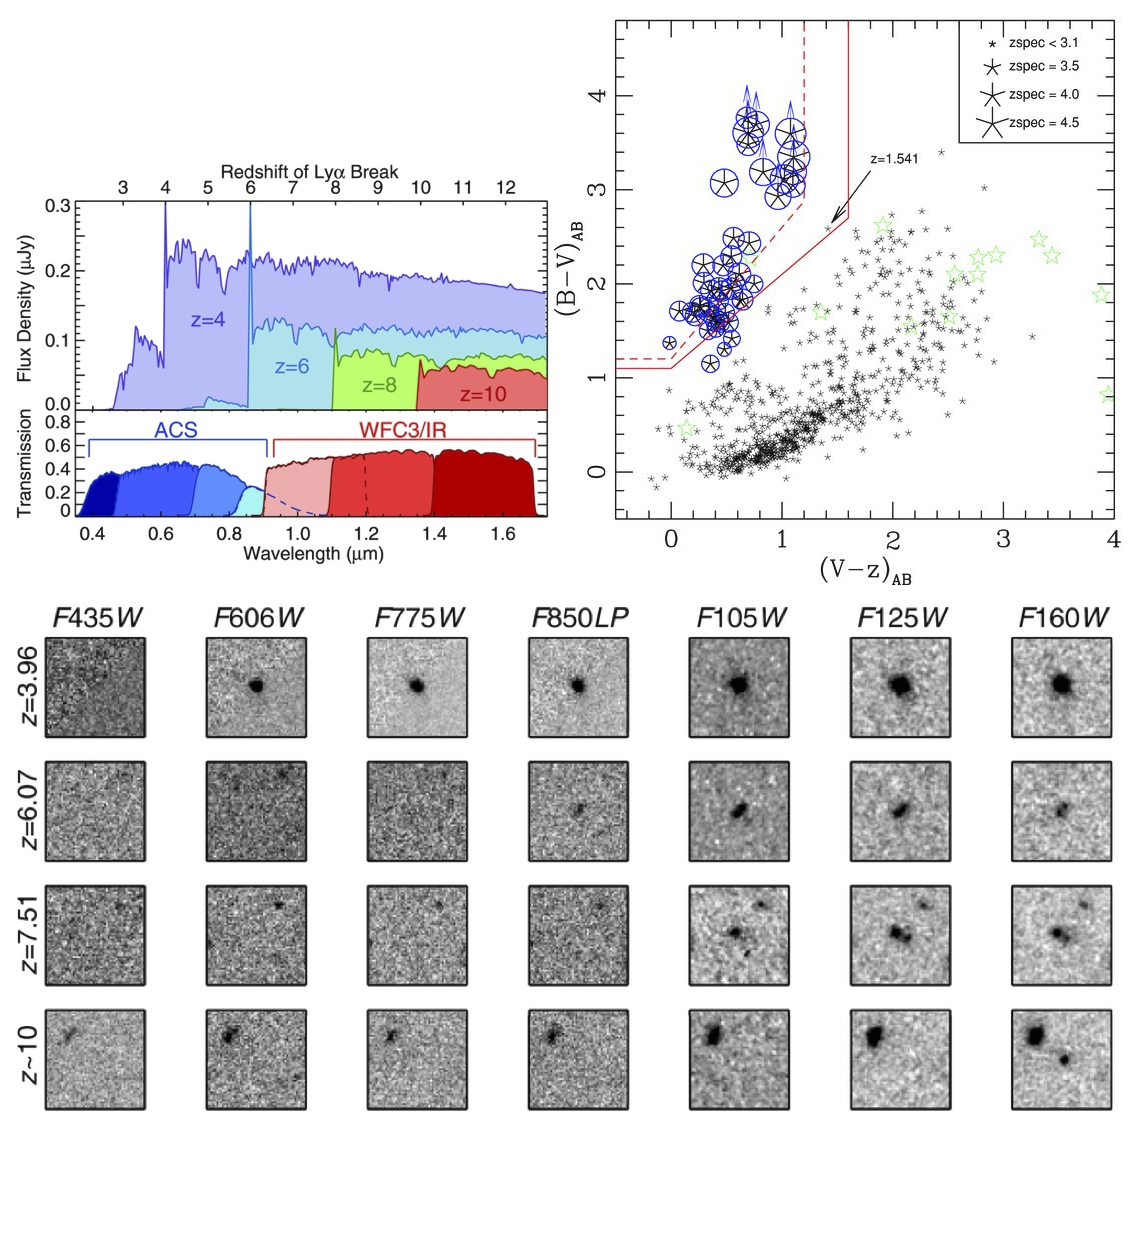
\includegraphics[width=1.0\textwidth]{Chapter1/Figs/Lyman_break_selection.png}
\caption[Selection of Lyman-break galaxies]{Illustration of the selection process for Lyman-break galaxies. The top left part is taken from \cite{2016PASA...33...37F}, and shows model spectra of star-forming galaxies at $z=4$, $z=6$, $z=8$, and $z=10$ together with the transmission curves for seven \textit{HST} filters. The bottom part, also adapted from \cite{2016PASA...33...37F}, consists of cutouts of \textit{HST} imaging showing real candidates in each of the aforementioned filters. It is clear that if the Lyman break lies between two filters, the galaxies show no flux (`drop out') in filters bluer than the Lyman break, but do appear in all redder filters. The top right figure is reproduced from \cite{2009ApJ...695.1163V}, and shows their colour-colour selection of $B$-dropouts (which lie at $3.1<z<4.4$) using the same filterset as the other two subfigures. The black markers indicate spectroscopically confirmed galaxies, with larger symbols denoting higher redshifts up to $z=4.5$. The green $\star$ symbols denote galactic stars, and the red box delineates the colour-colour cuts that were imposed to select $B$-drops. It is noteworthy that the only contamination inside the box consists of a single low-redshift galaxy (flagged by the arrow), thus demonstrating that the colour cuts lead to highly efficient selection.} 
\label{fig:lyman_break}
\end{figure}


For many star-forming galaxies, the Lyman break is strong enough to be observable in broadband imaging, especially if it falls between two filters. Such a galaxy will be visible in all filters redder than the Lyman break, while it will be undetected (it will `drop out') in all bluer filters. Because of this behaviour, such objects are often referred to as \textit{dropout} galaxies, and the first filter longwards of the Lyman break is often referred to as the \textit{detection} filter. Objects with a Lyman break between the $u$-band and $g$-band (or equivalently the $B$-band in other filter sets) are labelled $u$-dropouts. As their observed Lyman break lies between the $u$ and $g$ filter (roughly at $\lambda_{\mathrm{obs}}\simeq\SI{3500}{\angstrom}$, depending on the filter set), their redshift is approximately $z\sim3$. Using the exact same reasoning, $g$-dropouts (sometimes called $B$-dropouts) lie at $z\sim4$, $r$-dropouts (or $V$-dropouts) at $z\sim5$, and $i$-dropouts at $z\sim6$. The dropout mechanism is depicted in Figure \ref{fig:lyman_break}, which illustrates the appearance of Lyman-break galaxies at various redshifts. \par  

The simplest way to select galaxies via their Lyman break involves using colour cuts to select galaxies that show a red colour between the dropout band and the detection band (to confirm a strong Lyman break) and a blue colour between this detection filter and the next reddest band (to select blue star-forming galaxies rather than low-redshift galaxies or stars with intrinsically red colours). This technique is demonstrated in the top right of Figure \ref{fig:lyman_break}. \par 
 
Naturally, it is also possible to find dropout galaxies in a specific redshift range using photometric redshifts. At high redshifts, such a photo-z approach can often essentially be viewed as a form of Lyman-break selection. This is because at $z\gtrsim5$, the Balmer/\SI{4000}{\angstrom} break --- which is generally the second prominent spectral break --- has redshifted beyond the near-infrared. When using only broadband optical and near-IR data, the  Lyman break is therefore the only strong spectral feature that photo-z algorithms can use to estimate the redshift. Throughout this thesis, any galaxy selected via its broadband rest-frame UV colours will be referred to as a \textit{Lyman-break galaxy} (LBG). This includes objects selected via colour-colour cuts as well as via photometric redshifts. \par 

Colour selection methods and photometric redshifts each have their own merits. The colour-cut method is conceptually simple, computationally fast, not affected by specifics in the photo-z code (such as the template set), and highly reproducable. These advantages also make it more straightforward to model contamination and completeness rates for selected LBG samples, which is necessary for some statistical studies (e.g. the luminosity function introduced in Section \ref{subsubsection:photoz_galaxy_evolution} and to be  discussed further in Section \ref{subsubsection:high_redshift_galaxy_evolution}). On the other hand, colour cuts only make use of data in at most three filters, whereas the photo-z approach makes use of the full available dataset. Additionally, as indicated in Section \ref{subsection:methods}, some photometric redshift methods can also constrain certain galaxy properties, as well as output a redshift probability distribution for each source. The latter estimates the probability of potential low-redshift solutions, and also helps to increase the redshift precision (with photometric redshifts the precision at $z\sim6$ is around $\Delta z \sim \pm 0.2\text{--}0.3$, as opposed to $\Delta z \sim0.5$ for colour-cut techniques; \citealt{2016PASA...33...37F}). The history and current status of observational searches for LBGs will be discussed in Section \ref{subsubsection:lyman_break_galaxy_history}, where it will be shown that both photo-zs and colour cuts remain competitive up to the current day. The choice of method therefore largely depends on the research goals and available filtersets for each LBG study, and on the personal preference of the authors. \par  




\subsubsection{Quiescent and dusty high-redshift galaxies}\label{subsubsection:dusty_quiescent}
The selection of LAEs and LBGs described above is based on their rest-frame UV emission, which means that these methods are only sensitive to galaxies with active star formation that is not significantly attenuated by dust. Therefore, these strategies will miss extremely dusty galaxies, as well as passive quiescent galaxies that no longer form stars. \par 

However, an alternative search method that makes use of submillimeter imaging has revealed several highly dust-attenuated galaxies at $z\gtrsim5$ (see e.g. \citealt{2010ApJ...720L.131R,2012Natur.486..233W}). The UV radiation produced by the intense star formation in these extremely reddened objects is almost entirely absorbed by the vast amounts of dust in their interstellar media. This process heats the dust, which then re-radiates its energy at (rest-frame) far-infrared wavelengths. At high redshifts, this emission is shifted into the submillimeter regime, where it can be detected by instruments such as the \textit{Herschell Space Observatory} and the James Clerk Maxwell Telescope.  An in-depth discussion of extremely dusty galaxies is outside the scope of this thesis, but  \cite{2014PhR...541...45C} provide an excellent review for those who are interested in more information. \par 

Regarding quiescent galaxies, there are currently no known secure candidates\footnote{Although it must be noted that \cite{2016PASJ...68...46M} have found a number of uncertain contenders.} of this population at $z\gtrsim5$. While photometric redshifts and colour-colour cuts directed at the Balmer break\footnote{This method works analogously to the Lyman-break colour selection described in Section \ref{subsubsection:lyman_break}.} have yielded a handful of plausible candidates at $z\sim4.5$ \citep{2014ApJ...794...68N,2018MNRAS.473.2098M}, none of these are spectroscopically confirmed. The fact that searches have thus far not returned any convincing results is in fact not unexpected; since galaxies at $z>5$ would have needed to reach quiescence within 1.2 Gyr of the Big Bang, a large population of such objects is very unlikely. If they do indeed exist, the deep near-IR imaging that will soon be available with \textit{JWST} should be able to uncover them \citep{2016PASA...33...37F,2016PASJ...68...46M}. \par




\subsection{Lyman-break galaxies at high redshifts}
Out of all the different types of high-redshift galaxies discussed above, this thesis exclusively concerns itself with Lyman-break sources, for reasons that will be substantiated in Section \ref{section:motivation_high_z}. The rest of the current review of high-redshift science will therefore focus exclusively on this topic. The discussion will cover a brief overview of $z\gtrsim5$ LBG searches in the literature, as well as an outline of several interesting quantities and physical probes that can be studied via these objects. \par 

\subsubsection{Historical overview and state of the art}\label{subsubsection:lyman_break_galaxy_history}
The first attempts to identify distant galaxies by their Lyman break began at the start of the CCD era in the early 1990s \citep{1990ApJ...357L...9G,1993AJ....105.2017S}. These early studies used colour-colour cuts to select $u$-dropouts around $z\sim3$, and the first such candidate was soon spectroscopically confirmed \citep{1994A&A...288..103G}. By the end of the decade, small samples of galaxies were starting to be found around $z\sim5$, with the rapidly developing photo-z techniques providing a valuable tool in this endeavour \citep{1996Natur.381..759L,1999ApJ...513...34F}. A handful of these candidates quickly received spectroscopic confirmation \citep{1998AJ....116.2617S,1998ApJ...505L..95W}.  Nevertheless, larger samples of high-redshift galaxies could not be identified until the development of better red-sensitive instrumentation. After this need was met by new \textit{HST} instruments in the mid-2000s, space-based surveys such as GOODS and the HUDF (see Table \ref{table:space_small_survey} for both) started to unveil samples of more than a hundred $z>5$ galaxy candidates, discovered through either colour-cut or photometric redshift methods \citep{2003MNRAS.342..439S,2004ApJ...600L.103G,2006A&A...449..951G,2006ApJ...653...53B}. One of the first spectroscopic confirmations of a $z\sim6$ candidate followed soon after \citep{2004ApJ...600L..99D}. Around the same time, parallel improvements in terrestrial telescopes enabled significant progress from the ground. Surveys such as the SDF, SDXF (both optical, see Table \ref{table:ground_small_survey}), and UKIDDS (near-IR, idem) prompted the discovery of large samples of high-redshift LBGs from ground-based data, again using both colour cuts and photo-z selection. Although only just over twenty candidates were found at $z>7$ \citep{2009ApJ...706.1136O}, more than a hundred were discovered at $z\sim5$ and $z\sim6$ \citep{2004ApJ...613L...9N,2004ApJ...611..660O,2006MNRAS.372..357M,2006ApJ...653..988Y}. These ground-based searches covered areas of $\sim \SI{1}{\sqdeg}$ --- more than a two-fold increase over GOODS, the largest space-based project at the time. Since larger search areas are more likely to contain rare objects, these ground-based datasets complemented space-based imaging by revealing bright galaxies (<\SI{26.0}{\magab}), which are too uncommon for the relatively narrow surveys from space. \par


The last 10 years brought even further advancements in the selection of LBG samples. From space, improvements in instrumentation led to deeper and wider surveys\footnote{The CANDELS, HUDF09 and HUDF12 data have also been combined into the HXDF, which was introduced in Section \ref{subsubsection:space_based_surveys}.} such as CANDELS (see Table \ref{table:space_small_survey}), HUDF09 (PI: Illingworth, described in e.g. \citealt{2011ApJ...737...90B}), and  HUDF12 \citep{2013ApJS..209....3K}, which together yielded around 3000 $z\sim5$ and 800 $z\sim6$ LBG candidates \citep{2015ApJ...810...71F,2015ApJ...803...34B}. The extreme depths also allowed the selection of several hundred secure candidates out to $z\sim7\text{--}8$ \citep{2015ApJ...810...71F,2015ApJ...803...34B}, and roughly a few dozen\footnote{Among these is an object spectroscopically confirmed at $z=11.1$ \citep{2016ApJ...819..129O}. This galaxy is currently the most distant known source in the universe. As this implies that we are now able to observe a glimpse of the universe just 400Myr after the Big Bang, its discovery can certainly be regarded as a great triumph of extragalactic astronomy.} objects at $z\gtrsim9$ \citep{2013ApJ...773...75O,2014ApJ...786..108O,2015ApJ...803...34B}. Meanwhile, there similarly were significant advances from the ground, with surveys such as CFHTLS, UltraVISTA, and VIDEO (see Table \ref{table:ground_small_survey} for all) covering footprints of $>\SI{1}{\sqdeg}$. Those larger search areas opened up the study of the brightest ($z_{\mathrm{AB}}<25.0$) high-redshift candidates, which will be discussed in more detail shortly. They also revealed several dozen $z\sim7$ candidates \citep{2010A&A...524A..28C,2014MNRAS.440.2810B}, but the vast majority of ground-based objects were discovered at $z\sim5\text{--}6$, with a combined total of hundreds of plausible LBGs at $z\sim6$ \citep{2013AJ....145....4W,2015MNRAS.452.1817B,2009MNRAS.395.2196M} and thousands at $z\sim5$ \citep{2009MNRAS.395.2196M,2010A&A...523A..74V}. The reason why so many more $z\sim5$ candidates have been found compared to $z\sim6$, besides an intrinsic drop in number density with increasing redshift, lies partly in the available datasets. The underlying cause is that secure redshift estimates require detections in at least 2 bands redwards of the Lyman break\footnote{This is necessary to select galaxies with blue intrinsic colours, in order to remove contamination from intrinsically red objects such as dusty galaxies and low mass stars. This requirement applies to both photometric redshift methods and colour cuts, although in the case of photometric redshifts, more detections are additionally useful for providing a better constraint on the fit.}. Since many optical datasets include $i$- and $z$-band data, $r$-dropouts at $z\sim5$ can be found from optical data alone, since they can be detected in both $i$ and $z$. However, additional redder filters are required for $i$-dropouts at $z\sim6$, which means that these searches are restricted by the availability of deep near-IR data. \par 

Up until the current day, colour-cut methods and photometric redshift selection both remain competitive, and the studies mentioned above have used both approaches in roughly equal numbers. Out of all  the LBG candidates that all those searches have identified, more than a hundred $z\gtrsim5$ galaxies have so far been spectroscopically confirmed, mostly at $z<7$  (e.g. \citealt{2005ApJ...626..666M,2009ApJ...695.1163V,2010MNRAS.408.1628S,2011ApJ...743...65J,2012MNRAS.422.1425C,2014ApJ...793..113P,2018MNRAS.479...43K}). \par 

The picture that emerges from this collective body of research is rather impressive. Astronomers are now able to catch a first glimpse of the $z\gtrsim9$ universe, and statistically secure samples of hundreds of $z\sim7\text{--}8$ galaxies are beginning to emerge. The state of the art at $z\sim5$ and $z\sim6$ also contains a wealth of data, with over 1000 and \num{10000} candidates respectively. Nevertheless, despite all this progress, number counts of the brightest ($z_{\mathrm{AB}}<25.0$) LBGs at $z\sim6$ are still relatively low. At the time of writing\footnote{It is possible that the study by \cite{2015ApJ...810...71F} also contains some candidates, but they did not publish apparent magnitudes, and the footprint of their study is almost entirely contained within \cite{2015ApJ...803...34B}, so these results are omitted.}, there are 14 such candidates from a \SI{4}{\sqdeg} ground-based study by \cite{2013AJ....145....4W},  9 from a \SI{1.65}{\sqdeg}  ground-based search by \cite{2015MNRAS.452.1817B}, and approximately\footnote{It must be noted that these galaxies are classified as bright due to their $Y_{105}<25.0$ magnitude, as \cite{2015ApJ...803...34B} did not publish $z$-band magnitudes. Therefore it is possible that the actual number of $z<25.0$ slightly deviates from this number.} 13 from \SI{0.26}{\sqdeg} from a predominantly space-based investigation by \cite{2015ApJ...803...34B}. After accounting for duplicates, those studies contain a relatively modest total of 32 unique $z_{\mathrm{AB}}<25.0$ candidates. A combination of deep optical and near-IR imaging over a large area of several square degrees would be required to improve these numbers. \par





\subsubsection{The importance of Lyman-break galaxies for high-redshift galaxy evolution studies}\label{subsubsection:high_redshift_galaxy_evolution} %CALL THIS 'THE IMPORTANCE OF HIGH-REDSHIFT LYMAN-BREAK GALAXIES'
Samples of high-redshift Lyman-break galaxies from the last 20 years have contributed enormously to the study of galaxy evolution at early times. This is an extremely rich field with a vast quantity of ongoing research, and a detailed summary of recent developments can be found in the reviews by  \cite{2013ASSL..396..223D} and \cite{2016PASA...33...37F}. However, in order to provide a brief illustration of the interesting science that can be achieved with high-redshift LBGs, this section highlights\footnote{Since the target of this thesis is bright LBGs (for reasons that will be presented in Section \ref{subsection:conclusion_high_z_intro} shortly), the narrative will focus predominantly on those objects. More information on all the science that can be achieved with fainter sources can be found in e.g. \cite{2013ASSL..396..223D} and \cite{2016PASA...33...37F}.} a number of interesting galaxy properties that can be investigated through these objects. \par


\paragraph{UV luminosity function} One of the most straightforward quantities to measure from samples of Lyman-break galaxies is the UV luminosity function (LF; briefly introduced in Section \ref{subsubsection:photoz_galaxy_evolution} earlier), which quantifies the number density of galaxies per unit of comoving volume per unit of absolute rest-frame UV luminosity (usually $M_{\SI{1600}{\angstrom}}$ or $M_{\SI{1500}{\angstrom}}$). The reason why LBG LFs are usually measured in the ultraviolet is because the deepest survey data generally exists at optical and near-IR frequencies, which for LBG redshifts of $z\gtrsim3$ translates to the rest-frame UV.  \par


The UV luminosity function is an extremely useful measure, as it provides insights into physical processes in the universe. For instance, it can be used to estimate the total number of ionizing UV photons produced by galaxies, and thus whether galaxies could have been the main contributor to the reionisation of the intergalactic medium \citep{2010Natur.468...49R,2013ApJ...768...71R}. Furthermore, because it tracks light from newly formed blue stars, the UV luminosity function can also be converted into the cosmic star formation rate density, which quantifies the total amount of star formation occurring in the universe at a given redshift. Studying the variation of the cosmic star formation rate with redshift has started to provide some insights into the growth of stellar mass, and when its build-up commenced \citep{2013ApJ...763L...7E,2014ARA&A..52..415M,2015ApJ...803...34B,2015ApJ...810...71F}. Lastly, because it can be computed fairly easily from both theory and observations, the LF is a useful probe for some of the physical processes that drive galaxy evolution.  A comparison between the shape of the luminosity function (from observations) and the halo mass function of the underlying dark matter haloes (from simulations) can provide clues as to the physical mechanisms at play. At both the bright and the faint end, the luminosity function at most redshifts has generally been found to lie below what would be expected on the basis of galaxy halo masses. This suggests that the conversion of gas (the abundance of which roughly scales with the dark matter halo mass) into starlight is less efficient in both the brightest and the faintest galaxies. It is believed that this phenomenon is caused primarily by processes that heat the interstellar medium and expel gas from galaxies, which subsequently suppresses their star formation. The primary candidates for causing this disruption include supernova feedback and stellar winds at the faint end, and AGN feedback at the bright end \citep{2003ApJ...599...38B,2008MNRAS.391..481S,2015ARA&A..53...51S}.  \par


\begin{figure}[t] 
\centering    
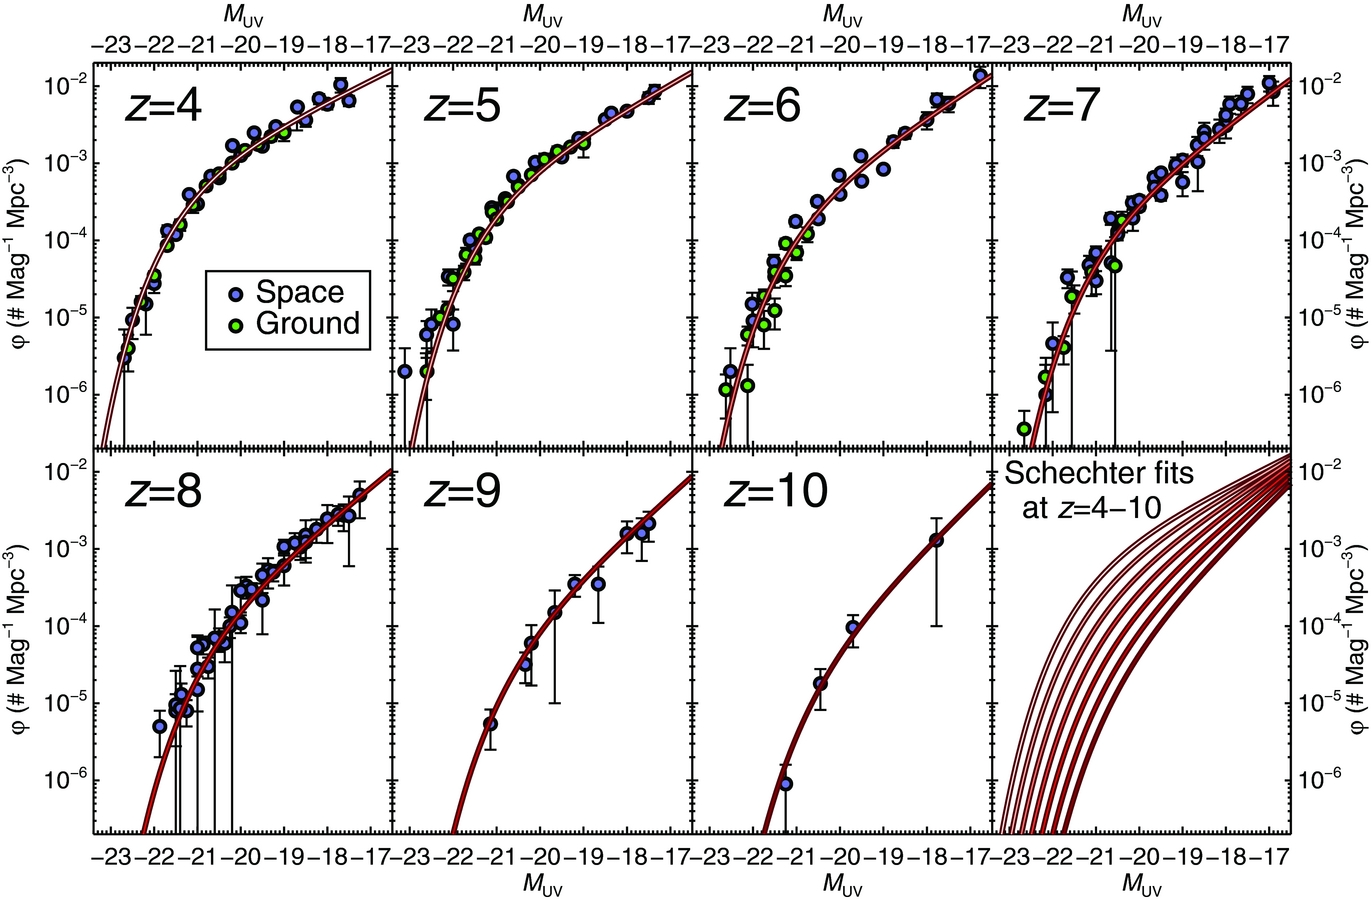
\includegraphics[width=1\textwidth]{Chapter1/Figs/Luminosity_functions.png}
\caption[Luminosity functions at \texorpdfstring{$4<z<10$}{TEXT}]{A compilation of UV luminosity functions created by \cite{2016PASA...33...37F}, constructed from recent samples of LBGs in various redshift bins. The dots are data points from several space-based and ground-based studies (sources are listed in \citealt{2016PASA...33...37F}), and the red curves are reference Schechter function \citep{1976ApJ...203..297S} fits to these data points (computed as described in \citealt{2016PASA...33...37F}).}
%It is clear that at $z\sim4$ and $z\sim5$ the luminosity functions are well constrained, with low scatter and low uncertainties, while at $z\gtrsim7$ the uncertainties are larger due to the smaller sample sizes. The situation at $z\sim6$ is mixed, with low uncertainties at the faint end\footnote{The scatter in the faint end at $z\sim6$ is caused by a difference in the normalisation factor due to systematic differences in the LF computation between studies (see \cite{2016PASA...33...37F})} and larger error bars at the bright end. These large uncertainties are predominantly caused by the small (<50) sample size of these bright objects (see Section \ref{subsubsection:lyman_break_galaxy_history}).
\label{fig:luminosity_functions}
\end{figure}


To study the changes in all these physical processes over time, UV luminosity functions are usually computed from samples of LBGs at various redshifts. In order to be able to reach secure conclusions, it is important that these functions are well measured. To illustrate to what extent current data provide adequate constraints, Figure \ref{fig:luminosity_functions} shows a compilation of LF data points from recent observational studies at $4<z<10$. It is clear that the measurements at $z\sim4$ provide fairly solid constraints, thanks to the generous samples of LBGs used to obtain these data points. Similarly, it is evident that the same largely applies at $z\sim5$ (with the exception of the extreme bright end, which shows some large error bars mainly due to space-based studies having low number counts in this regime). And conversely, it is also apparent that the results at $z\gtrsim7$ are generally rather uncertain, primarily due to the small sample sizes. The data points at $z\sim6$, on the other hand, present a more mixed situation. At the faint end, the uncertainties are small, although there does exist some scatter (likely originating from systematic differences in the LF computation between studies; \citealt{2016PASA...33...37F}). The bright end likewise suggests some tension between studies, but critically shows much larger error bars in addition to that. Those big uncertainties are predominantly caused by the small number of known bright galaxies, an issue which has previously been noted in Section \ref{subsubsection:lyman_break_galaxy_history}. Better constraints in this regime would be valuable, since the bright end around $z\sim6$ also happens to be especially interesting scientifically. This is because there are indications that the aforementioned drop in bright sources compared to the halo mass function, which is known to exist at lower redshifts (e.g. \citealt{2010A&A...523A..74V}), may have commenced around this time \citep{2014MNRAS.440.2810B,2015MNRAS.452.1817B}. This could indicate the start of processes that suppress star formation (such as the beginning of AGN activity), or the onset of dust build-up that obscures some of the stellar UV radiation (see \citealt{2012ApJ...756..164F,2014ApJ...793..115B,2014MNRAS.440.3714R}). \par 


\paragraph{Other galaxy properties}
In addition to the UV luminosity function, there are several other important physical attributes that can be studied with the help of high-redshift LBGs. A major one of these is their stellar masses, which can be probed if mid-IR \textit{Spitzer Space Telescope} data is available  \citep{2006ApJ...651...24Y,2009ApJ...697.1493S,2010ApJ...719.1250F,2011ApJ...735L..34G}. Such imaging captures the rest-frame optical emission, which, in contrast to the rest-frame UV, is sensitive to lower-mass stars that may make up the bulk of galaxy mass. As well as for its own sake, stellar mass has been used to study the amount of star formation in a galaxy per unit of stellar mass (the specific star formation rate; \citealt{2013ApJ...763..129S,2014ApJ...781...34G,2015ApJ...799..183S}) and the dependence of galaxy stellar masses on the underlying dark matter halo mass \citep{2009MNRAS.395.2196M,2013ApJ...770...57B,2015ApJ...814...95F}. Dust attenuation is another interesting property that is being studied, as there is a reasonable amount of evidence that out to $z\sim7$ the brightest galaxies already contain an appreciable amount of dust (displaying reddening of $E(B-V)\sim 0.1\text{--}0.15$; \citealt{2012ApJ...754...83B,2014ApJ...793..115B,2012ApJ...756..164F,2014MNRAS.440.3714R,2015ApJ...814...95F}). Finally, some authors have also begun to make small steps to measure the evolution of galaxy sizes \citep{2010ApJ...709L..21O,2013ApJ...765...68H,2013AJ....145....4W,2014MNRAS.440.2810B}. \par

Spectroscopic follow-up of high-redshift LBG candidates can also provide interesting physical insights, since spectra can  be used to measure the possible presence and strength of the Lyman-$\alpha$ emission line. This can provide constraints on reionisation: if galaxies beyond a certain redshift show an average reduction in their Lyman-$\alpha$ flux, this could signal the presence of increased neutral hydrogen in the IGM (and hence incomplete reionisation). Recent studies indicate that such a drop in Lyman-$\alpha$ has indeed been observed around $z>6$ \citep{2010MNRAS.408.1628S,2011ApJ...743..132P,2013Natur.502..524F,2014ApJ...793..113P}, which agrees with the current consensus that reionisation ended around $z\approx6$. The specifics of how the reduction in Lyman-$\alpha$ at $z>6$ can be converted into particular details about the progression of reionisation are currently the topic of active debate, and there are some tensions between theory and observation (see e.g. the reviews by \citealt{2014PASA...31...40D} and \citealt{2016PASA...33...37F}, and references therein). While spectroscopy at $z>6.5$ would provide the most useful constraints, this is challenging with most instruments due to the dramatic reduction in the sensitivity of optical spectrographs at the extreme red end. However, spectra of $z\approx6$ galaxies are easier to obtain and would also be useful. For instance, galaxies at $z\approx6$ can be used to extrapolate the Lyman-$\alpha$ equivalent width and escape fraction at $z>6.5$ in the absence of neutral hydrogen \citep{2009ApJ...697.1493S,2011ApJ...728L...2S}. This baseline can then be compared to the observed signature from real $z>6.5$ galaxies to estimate how much (not-yet-ionised) neutral hydrogen gas is present in the IGM. There is evidence that the Ly$\alpha$ escape fraction and equivalent width decrease with luminosity, but for the brightest sources the uncertainties on this hypothesis are still large due to the small number counts \citep{2009ApJ...697.1493S,2011ApJ...728L...2S,2012MNRAS.422.1425C}. More spectra of luminous $z\approx6$ objects would therefore be useful. At these great distances, bright galaxies are also more likely to yield usable spectra, making them very suitable targets.  \par


\subsection{Conclusion on high-redshift galaxies}\label{subsection:conclusion_high_z_intro}
In the review above, which focused primarily on Lyman-break galaxies, we have witnessed some key developments in recent high-redshift galaxy evolution studies. Along the way, the discussion presented a strong case in favour of collecting larger samples of the brightest ($z_{\mathrm{AB}}<25.0$) galaxies at $z\sim6$ in particular. For these objects, it was found that the current sample sizes are still small, which leads to large uncertainties on statistical properties. We observed several areas where bright LBG candidates would be valuable for future science. First and foremost, they are required to better constrain the bright end of the luminosity function, which can provide interesting clues as to the onset of AGN activity or dust build-up in the early universe. On top of that, they can also be used to investigate other physical properties, such as galaxy stellar mass and dust content. Finally, if spectra can be obtained, the Lyman-$\alpha$ emission of bright sources can help to provide further constraints on reionisation. \par 

The issue with the small number counts of known bright galaxies is largely caused by the relatively modest footprints of previous optical+near-IR surveys, which did not cover a large enough deep area to find substantial numbers of these rare sources. However, with an effective search area of \SI{4.9}{\sqdeg} ($7.5\sigma$ depths of $z_{\mathrm{AB}}<25.0$), the new optical+near-IR catalogue presented in this thesis offers the largest deep search area to date. Since its footprint only partially overlaps with the previous largest \SI{4}{\sqdeg} study by \cite{2013AJ....145....4W}, it
can provide an appreciable increase in potential sources. Armed with this new dataset, the third part of this thesis thus tackles the important task of identifying additional bright high-redshift Lyman-break galaxies. The largest scientific potential lies in sources at $z\sim6$; but since the dataset is also suitable for objects at $z\sim5$ those sources are also investigated, as we have seen that the extreme bright end of the LF at that redshift does still show considerable uncertainties. The high-redshift samples from these searches will be very valuable for future studies, for instance to help address some of the open questions regarding galaxy properties mentioned in the previous paragraph and Section \ref{subsubsection:high_redshift_galaxy_evolution}. \par




\section{Thesis outline}
Altogether, the current chapter has covered three important and related research areas in contemporary astronomy: surveys, photometric redshifts, and high-redshift galaxies. Each of these topics corresponds to one chapter of this thesis, and the main aims of each part have already been identified in the intermediary conclusions of each section (i.e. Sections \ref{subsection:conclusion_surveys_intro}, \ref{subsection:conclusion_photoz_intro}, and \ref{subsection:conclusion_high_z_intro}). A more detailed structural outline of this thesis is given below: 


\begin{itemize}
    \item \textbf{Chapter \ref{chapter:catalogue}} will address the creation of a \textbf{combined optical and near-infrared source catalogue}. The first section of this chapter will introduce the datasets for this thesis, which consist of the optical ($grizY$) Dark Energy Survey (DES) deep fields, the near-IR ($ZYJHK_{s}$) Vista Deep Extragalactic Observations (VIDEO) survey, and a catalogue of publicly available spectroscopic redshifts for a subset of these sources. The second section will then describe the process of combining the DES and VIDEO datasets into a single multiwavelength catalogue. This is achieved by creating a pipeline that extracts VIDEO forced photometry directly from the imaging and merges it with pre-existing DES collaboration catalogues. The third section will address accuracy verification for the resulting combined \DESVIDEO catalogue, and conclude with an overview of the final photometric data product.
    
    \item \textbf{Chapter \ref{chapter:photometric_redshifts}} will discuss the computation of \textbf{photometric redshifts for the ($grizZYJHK_{s}$) \DESVIDEO catalogue}. The first part will present the template fitting method \texttt{LePHARE} as the choice of code, and describe the working of this algorithm together with its various options and the relevant template SEDs. The second part will then introduce various \texttt{LePHARE} configurations for testing different templates, \texttt{LePHARE} options, and photometry. Each setup is used to compute photo-zs for a subset of \DESVIDEO objects with spectroscopic redshifts, and the photo-z performance of these test runs is assessed via a number of accuracy metrics that capture the difference between photometric and spectroscopic redshift. The primary purpose of this analysis is to identify the most suitable configuration to compute redshifts for the high-redshift search in Chapter \ref{chapter:high_redshift_candidates} (see below), but the discussion will also address the implication of the test results for general photo-z research. The final part of the chapter will then focus on  applying the chosen configurations to the full \DESVIDEO catalogue. This section will also discuss finding an appropriate star-galaxy separation strategy to filter out nonsensical photo-zs from stars, before finally presenting the final redshifts for all galaxies in the \DESVIDEO dataset. 
    
    \item \textbf{Chapter \ref{chapter:high_redshift_candidates}} will describe the \textbf{search for bright $\mathbf{z\sim5}$ and $\mathbf{z\sim6}$ Lyman-break galaxies in the \DESVIDEO catalogue}. The first part will discuss identifying a suitable strategy to select a sample of $m_{\mathrm{AB}} < 25.0$ candidate LBGs at $z\sim5$ and $z\sim6$, detailing the three selection rounds used in this search. The second part will then present the resulting final LBG sample, and compare the outcomes to other studies in the literature. 
\end{itemize}
